% For full compilation to get the final document
\documentclass[a4paper, 10pt]{article}

% For quick compilation without figures
% \documentclass[a4paper, 10pt, draft]{article}
\usepackage{float}
\usepackage{listings}
\usepackage{todonotes}
\usepackage{braket}
\usepackage{mathtools}
\usepackage[mathscr]{euscript}
\usepackage{amsmath, amsfonts, amssymb, amsbsy, amsthm}

\theoremstyle{plain}
\newtheorem{theorem}{Theorem}
\newtheorem*{theorem*}{Theorem}
\newtheorem{definition}[]{Definition}
\newtheorem{lemma}[]{Lemma}
\renewcommand\thelemma{\unskip}
\renewcommand\thedefinition{\unskip}
\renewcommand{\qedsymbol}{$\blacksquare$}

\usepackage{hyperref}
% \hypersetup{
%             colorlinks = true,
%             linkcolor  = blue,
%             filecolor  = magenta,
%             urlcolor   = blue
%            }
\urlstyle{same}

% Just to do labels in gnuplot, Yeah!
\usepackage{graphicx}
\usepackage{gnuplottex}
\usepackage{gnuplot-lua-tikz}


% ------------------------------------------------------------------------------
% Personal definitions
% ------------------------------------------------------------------------------
% Redefining the \abs and \norm so that they automatically change their size
\DeclarePairedDelimiter\abs{\lvert}{\rvert}%
\DeclarePairedDelimiter\norm{\lVert}{\rVert}%

% Swap the definition of \abs* and \norm*, so that \abs and \norm resizes the
% size of the brackets, and the starred version does not.
\makeatletter
    \let\oldabs\abs
    \def\abs{\@ifstar{\oldabs}{\oldabs*}}
%
    \let\oldnorm\norm
    \def\norm{\@ifstar{\oldnorm}{\oldnorm*}}
\makeatother
% ------------------------------------------------------------------------------


%opening

\begin{document}
\pagenumbering{gobble}
\begin{titlepage}

\begin{center}
%\onehalfspacing
%\doublespace
{\Huge \textbf{Thermalisation of}}\\[5mm]
{\Huge \textbf{Ultracold Bose Gases}}\\[5mm]
{\Huge \textbf{on Optical Lattices}}
\vspace*{3cm}

\Huge{Nikolas M. Mitchell}
\vspace*{35mm}

\Large{September 2017}
\vspace*{15mm}

\large{A dissertation submitted in partial fulfilment for  \\
the degree of Bachelor of Science with Honours in Physics}
\vfill

\includegraphics[width=0.2\textwidth]{OtagoLogo.eps}

\end{center}

\end{titlepage}

\begin{abstract}
    Systems of ultra-cold gases in light-induced periodic potentials, often
    called optical lattices, are of great experimental and theoretical interest,
    and have been since the first experimental realisation of Bose-Einstein
    condensation in 1995. This is largely due to the parallels between the
    behaviour of Bose-Einstein condensates in optical lattices and condensed
    matter systems, where electrons can be modelled as moving on a lattice
    generated by the periodic array of atom cores. This project investigates the
    time evolution of a system of bosons prepared in a far-from-equilibrium
    state on a one-dimensional or two-dimensional optical lattice. 
    
    We take two
    different approaches to this problem, employing a more exact many-body 
    approach to investigate smaller systems and then using the Gross-Pitaevskii 
    equation to extend our range of inquiry to include larger ones. The main
    focus is on determining how the tunnelling energies and the strength of the
    interparticle interactions influence whether or not the system exhibits
    relaxation to a thermal state. For systems in which revival to the initial
    state occurs regularly, and which thus do not seem to thermalise, a method for
    calculating the revival period is developed. For the systems which exhibit
    thermalisation, we attempt to characterise the thermal states using long 
    term averages of the expectation values of observables.
\end{abstract}
\newpage
\section*{Acknowledgements}
\thispagestyle{plain}
I would first like to thank my supervisor, David Hutchinson, for providing 
guidance and clear direction throughout the project, as well as unremitting
interest and encouragement. I would also like to thank John Helm, for 
his patient explanations of coding for the Gross-Pitaevskii approach taken 
in part of this dissertation. Thank you to my fellow inmates in the Honours 
room - your banter and camaraderie have brought enjoyment to many a long and 
busy day. Finally and especially, I would like to thank Daniel Schumayer -
your incredible generosity with your time and unshakeable good humour have been
invaluable.
\newpage
\tableofcontents
\newpage
\pagenumbering{arabic}
\section*{Introduction}
The question of how, and under what conditions, closed quantum systems approach
thermal equilibrium is an old question that forms the basis of a large and
active field of research. Thermalisation is well understood in the context
of classical mechanics, where it emerges from the chaotic
dynamics of sufficiently unconstrained systems. However, the time evolution of
quantum systems is strictly linear, and hence they do not exhibit chaotic
dynamics. Nonetheless, there are a number of closed quantum systems in which
thermalisation is observed, in the sense that the systems relax to states in
which the values of macroscopic quantities are stationary, universal with
respect to widely differing initial conditions, and predictable using
statistical mechanics \cite{Rigol2008}.

This project investigates the time evolution of a variety of different systems
composed of noninteracting and interacting bosons on one-dimensional and
two-dimensional optical lattices that are prepared in far-from-equilibrium
states. These systems are investigated analytically where possible, and with
numerical methods for larger and more complicated systems where an analytic
approach is not tractable. 

We focus primarily on gaining a strong
understanding of smaller systems of few lattice sites and bosons, as these
can be solved exactly. From here, we look at some larger systems with a more
approximate method that revolves around using an adaptive Runge-Kutta-Feldberg
method to evolve the system wavefunction according to the Gross-Pitaevskii
equation. We then look for similarities in the results of the simulations run
according to each method to see what how much of the behaviour of small,
exactly solved systems is preserved is we move to large, numerically approximated
systems. By doing so, we aim to pave the way for a systematic study of the role
of integrability in relaxation and thermalisation of far-from-equilibrium
quantum systems.
\newpage


\section{Experiments with optical lattices}

This project considers the thermalisation behaviour of systems of bosons on
optical lattices. One of the main factors that make these systems interesting
to work with are the deep similarities between the Hamiltonians of systems that
can be generated using bosons on an optical lattices and those of electrons
moving on a lattice potential produced by a periodic array of atom cores. We can
simulate these condensed matter systems with ultracold atoms by using optical
lattices to generate the periodic potential. An optical lattice is produced by
overlapping multiple laser beams and making use of the interference pattern.
The alternating bright and dark areas of the interference pattern act as a
periodic potential on the atoms through the optical dipole force
\cite{Bloch2012}. By superimposing different combinations of laser beams at
particular frequencies and amplitudes, any lattice geometry that can be
constructed via Fourier synthesis can, in principle, be produced
\cite{Bloch2012}. This fine degree of control over the lattice parameters, in
conjunction with the ability to tune the strength of interparticle interactions
by manipulating Feshbach resonances \cite{Chin2010}, makes ultracold bosons on
optical lattices an excellent arena in which to explore various model
Hamiltonians for condensed matter systems and quantum optics.
\begin{figure}[bh!]
    \begin{center}
        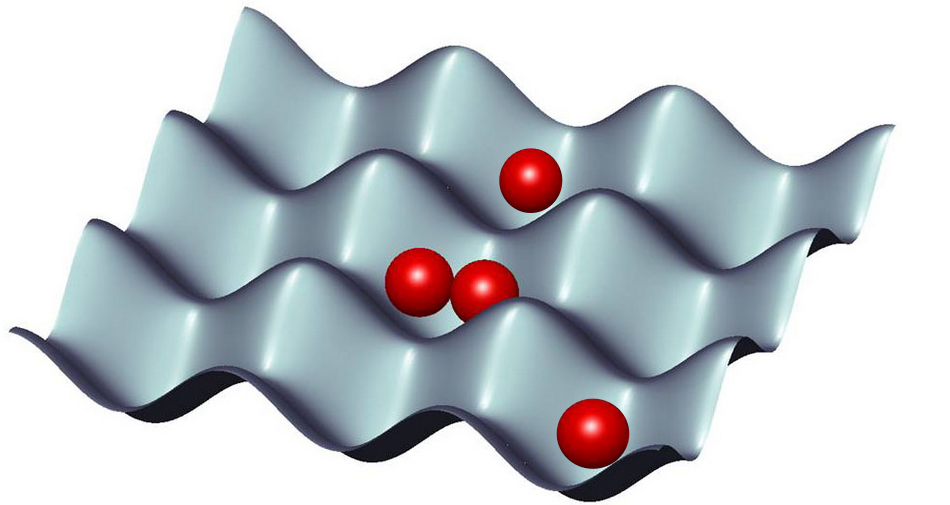
\includegraphics[width=8cm]{bosons_on_lattice}
    \end{center}
    \caption{Bosons on a two-dimensional optical lattice. Figure is taken from\newline
             \texttt{www.uibk.ac.at/th-physik/qo/research/opticallattices.html.en}
            }
\end{figure}
There are further advantages which can make conducting experiments with
ultracold bosons on optical lattices more attractive than working with solids
directly. One is that there are always impurities present in the solids we find
in nature. These impurities can have significant impacts on the properties of
the solid which cannot necessarily be accounted for by a perturbative approach
which assumes these effects to be small. For large-enough detunings from an atomic
transition frequency, optical lattices can be considered to be purely
conservative and defect-free potentials \cite{Bloch2012}, so when dealing with
bosons on optical lattices this problem of impurities does not arise.

Another benefit of working with bosons on optical lattices is that we can easily
control the state of each of the particles on the lattice. Furthermore, the
potential can be altered or switched off entirely during the experiment, which
is a feature that is not available in any solid state experiment
\cite{Morsch2006}.


\section{First quantised representation}

This dissertation will deal exclusively with bosons on optical lattices, and not
investigate cases involving fermions. There are a number of different
contributions to the Hamiltonian for bosons on optical lattices, and these
contributions can be seen to have analogues in condensed matter systems. The
individual bosons will have kinetic energy, and the potential created by the
lattice also contributes to how the system evolves in time, so it must feature
in the Hamiltonian. The bosons may be interacting, and there may also be an
external potential imposed that can vary in strength from site to site.

With regards to the interparticle interactions, we consider repulsive scattering
interactions. We will consider systems that are dilute, in the sense that the
average spacing between bosons is much greater than the effective range of the
interparticle interactions. This makes it reasonable to consider only
two-particle scattering events and neglect the rare higher order collisions,
provided we keep the strength of the interparticle interactions small. Even when
reduced to its two-body form, $U(x,x')$, the form of the interatomic scattering
potential has short range terms that can be difficult to deal with. We can
replace this object with a mathematically more convenient effective potential,
corresponding to contact interaction, with the same scattering cross-section at
low-energy. Because the ultracold bosons have such low energy, $s$-wave
scattering dominates, and the interparticle interaction potential can be
expressed simply in terms of the $s$-wave scattering length, $a_{s}$, as
\begin{equation}
    U_{\text{eff}}
    =
    \frac{2 \pi\hbar^{2} a_{s}}{m}
    \sum_{i,j}{\delta(x_{i} - x_{j})}.
\end{equation}
For simplicity, we will introduce the notation $U_{0} = \frac{4 \pi \hbar^{2}
a_{s}}{m}$. Having made these simplifications, we can construct a first
quantised Hamiltonian for a one-dimensional system of interacting bosons on an
optical lattice, in the presence of an external potential $V_{\text{ext}}$
\begin{equation}
    \label{eq:HamiltonianCoordinateRepresentation}
    \hat{h}
    =
    \sum_{i}{-\frac{\hbar^{2}}{2m}  \partial_{x_{i}}^{2}} +
    \sum_{i}{V_{\text{lattice}}(R_{i})} +
    V_{\text{ext}}(x) +
    \frac{U_{0}}{2} \sum_{i,j}{\delta(x_{i} - x_{j})}.
\end{equation}
Similar Hamiltonians are frequently used to describe systems of electrons on
atomic lattices. To promote conciseness, we introduce the abbreviations
\begin{equation*}
    \hat{h}_{1}
    =
    \sum_{i}{-\frac{\hbar^{2}}{2m} \partial_{x_{i}}^{2}} +
    \sum_{i}{V_{\text{lattice}}(R_{i})},
    \quad
    \hat{h}_{\text{ext}}
    =
    V_{\text{ext}}(x),
    \quad
    \hat{h}_{\text{int}}
    =
    \frac{U_{0}}{2} \sum_{i,j}\delta{(x_{i}-x_{j})}
\end{equation*}
so that $\hat{h}=\hat{h}_1+\hat{h}_{\text{ext}}+\hat{h}_{\text{int}}$.


\section{Effect of indistinguishability}

The Hamiltonian in the previous section would act on a bosonic many-particle
wave function. A single particle wave function $\psi(\mathbf{r})$ is defined
within a Hilbert space $\mathcal{H}$, which is the space of complex, square
integrable functions. It must satisfy $\int{d^3\mathbf{r}
\abs{\psi(\mathbf{r})}^{2}} < \infty$. A wave function that represents the state
of $N$ indistinguishable particles, $\psi(\mathbf{r}_{1}, \mathbf{r}_{2}, \dots,
\mathbf{r}_{N})$ is defined within $\mathcal{H}^N$, where $\mathcal{H}^N$ is
constructed as the tensor product $N$ single-particle Hilbert spaces:
\begin{equation}
    \mathcal{H}^{N} =
    \mathcal{H} \otimes \mathcal{H} \otimes \dots \otimes \mathcal{H}.
\end{equation}
The wave functions in this space are also subject to normalisation constraints,
i.e.,
\begin{equation*}
    \int d^{3} \mathbf{r}_{1} d^{3}\mathbf{r}_{2} \dots d^{3}\mathbf{r}_{N}
        \abs{\psi(\mathbf{r}_{1},\mathbf{r}_{2},\dots,\mathbf{r}_{N})}^{2}
    < \infty.
\end{equation*}
Whilst all functions satisfying the above constraints can be legitimately
defined mathematically, only a small subset are found to occur in nature --
those which are either entirely symmetric or anti-symmetric under particle
exchange. The set of indistinguishable particles which are entirely symmetric
under particle exchange are called bosons. This project will not investigate
scenarios involving the particles that display exchange anti-symmetry
(fermions), so we will be working within the space $S_{N}\mathcal{H}^{N}$. Here
$S_{N}$ projects onto the subspace of square-integrable functions that are
unchanged by permuting the order of the variables. As an illuminating example
one may construct the two-particle space, $S_{2}\mathcal{H}^{2}$ for bosons as
\begin{equation*}
    S_{2} \mathcal{H}^{2}
    =
    \left \lbrace
        \psi \mid \psi = \psi_{1} \otimes \psi_{2} + \psi_{2} \otimes \psi_{1},
        \quad \text{where }\, \psi_{1}, \psi_{2} \in \mathcal{H}
    \right \rbrace
\end{equation*}
It is apparent that $S_{2} \mathcal{H}^{2} \ne \mathcal{H} \otimes \mathcal{H}$
since in this case we would be able to distinguish particles or states.
We can formally extend this notion of exchange symmetry for larger systems and
express the requirement of exchange symmetry for bosonic systems as
\cite{Negele1988}
\begin{equation*}
    \psi({\mathbf{r}_{\mathcal{P}_1}, \mathbf{r}_{\mathcal{P}_2}, \dots,
          \mathbf{r}_{\mathcal{P}_N}})
    =
    \psi(\mathbf{r}_{1}, \mathbf{r}_{2}, \dots, \mathbf{r}_{N}),
\end{equation*}
where $\lbrace \mathcal{P}_{1}, \mathcal{P}_{2}, \dots, \mathcal{P}_{N} \rbrace$
represents any permutation, $\mathcal{P}$, of the set $\lbrace 1, 2, \dots, N
\rbrace$.

Let us first consider the case of two indistinguishable bosons. We have not yet
determined the energy eigenstates of our Hamiltonian, but if we suppose we have
the set of normalised single-particle wave functions $\lbrace \ket{\lambda}
\rbrace$, and we have one boson in state $\ket{\lambda_1}$ and another in state
$\ket{\lambda_2}$, then we can write the two-particle wave function as
\begin{equation}
    \psi(\mathbf{r}_{1},\mathbf{r}_{2})
    =
    \frac{1}{\sqrt{2}}
    \big (
        \braket{\mathbf{r}_{1} | \lambda_1} \braket{\mathbf{r}_{2} | \lambda_2} +
        \braket{\mathbf{r}_{1} | \lambda_2} \braket{\mathbf{r}_{2} | \lambda_1}
    \big ),
\end{equation}
or in Dirac bra-ket notation, the two-body states would be represented as
\begin{equation}
    \ket{\lambda_1, \lambda_2}
    =
    \frac{1}{\sqrt{2}}
    \big (
        \ket{\lambda_1} \otimes \ket{\lambda_2} +
        \ket{\lambda_2} \otimes \ket{\lambda_1}
    \big ).
\end{equation}

The number of permutations that one must account for grows extremely quickly as
particle number increases. A properly symmetrised and normalised $N$-body state
can be represented \cite{Altland2010} as
\begin{equation}
    \ket{\lambda_{1}, \lambda_{2}, \dots, \lambda_{N}}
    =
    \frac{1}{\sqrt{N! \prod_{\lambda = 0}^{\infty}{n_{\lambda}}}}
    \sum_{\mathcal{P}}
        \ket{\lambda_{\mathcal{P}_{1}}} \otimes
        \ket{\lambda_{\mathcal{P}_{2}}} \otimes
        \dots                         \otimes
        \ket{\lambda_{\mathcal{P}_{N}}},
\end{equation}
where $n_{\lambda}$ is the number of particles in state $\lambda$, and the
summation runs over all $N!$ permutations $\mathcal{P}$ of the set of quantum
numbers $\lbrace \lambda_{1}, \dots, \lambda_{N} \rbrace$.

This formalism has a number of shortcomings. The most important of these for
this project is that it is extremely cumbersome for practical computation
because of the large number of entities that need to be represented. To avoid
this, we shall adopt the second quantised formalism, which is much better suited
to dealing concisely with large numbers of indistinguishable particles.

\section{Second Quantisation}

\subsection{The Occupation Number Representation}

The formalism that we have hitherto discussed explicitly represents a
significant amount of redundant information, in the sense that it deals
separately with the scenarios ``particle 1 in state $\lambda_1$ and particle 2
in state $\lambda_{2}$'' and ``particle 2 in state $\lambda_1$ and particle 1 in
state $\lambda_{2}$''. Taking into account the indistinguishability of the
particles, it is clear that these two scenarios are identical. A more efficient
approach consists of describing the number of particles in a particular state
$\lambda_i$, i.e., using the occupation number representation. When doing this,
a general state can be written as a linear superposition
\begin{equation}
    \ket{\Psi}
    =
    \sum_{n_{1}, n_{2}, \dots}%
        {c_{n_{1}, n_{2}, \dots}\ket{n_{1}, n_{2}, \dots}}.
\end{equation}
In the scenario which this project will be working with, the occupation numbers
refer to the number of bosons on a particular site of the lattice. Having
established this, we can define creation and annihilation operators that create
and annihilate particles from number eigenstates, that is
\begin{equation}
    \hat{a}_{j}^{\dagger} \ket{n_{1}, n_{2}, \dots, n_{j}, \dots}
    =
    \sqrt{n_{j} + 1} \ket{n_{1}, n_{2}, \dots, n_{j}+1, \dots}
\end{equation}
and
\begin{equation}
    \hat{a}_{j} \ket{n_{1}, n_{2}, \dots, n_{j}, \dots}
    =
    \sqrt{n_{j}} \ket{n_{1}, n_{2}, \dots, n_{j}-1, \dots}.
\end{equation}
These operators have very important commutation relations
\begin{equation}
    [ \hat{a}_{j}^{\dagger}, \hat{a}_{k}^{\dagger}] = 0, \quad
    [ \hat{a}_{j}, \hat{a}_{k}]=0, \quad
    [\hat{a}_{j},\hat{a}_{k}^{\dagger}]=\delta_{jk}.
\end{equation}
We can also define the number operator $\hat{n}_{j} = \hat{a}_{j}^{\dagger}
\hat{a}_{j}$ that has the property that
\begin{equation}
    \hat{n}_{j} \ket{n_{1}, n_{2}, \dots, n_{j}, \dots}
    =
    n_{j} \ket{n_{1}, n_{2}, \dots, n_{j}, \dots}.
\end{equation}

The occupation number eigenstates form the basis of the $N$-particle Hilbert
space that we are working in (the Fock space $\mathcal{F}^N$), and it is useful
to observe that any occupation number eigenstate can be created from the empty
(or ``vacuum'') state $\ket{0}$ by repeated action of
creation operators \cite{Altland2010}
\begin{equation}
    \ket{n_{1}, n_{2}, \dots}
    =
    \prod_{i}{\frac{1}{\sqrt{n_{i}!}}(\hat{a}_i^{\dagger})^{n_{i}}} \ket{0}.
\end{equation}
It may seem that the state space $S_{N}\mathcal{H}^N$ that we have constructed
is not robust enough to accommodate these operators. Indeed, the creation and
annihilation operators take us from the $N$-particle Hilbert space to the
$(N+1)$- and $(N-1)$-particle Hilbert spaces, respectively. In order to account
for these differences in particle number, we must really be working within the
symmetric Fock states $\mathcal{F}_{S}(\mathcal{H})$, defined by the direct sum
\cite{Blank1999}
\begin{equation}
    \mathcal{F}_{S}(\mathcal{H}) = \oplus_{N=0}^\infty S_{N} \mathcal{H}^N.
\end{equation}
However, we will be working in systems in which the particle number is
conserved. Each combination of creation and annihilation operators that appears
in the Hamiltonian will create an equal number of particles to the number
destroyed. So for practical purposes we are just working within $S_{N}
\mathcal{H}^{N}$.

Having established the space and states that we are operating with, we now need
to rewrite the Hamiltonian in number state representation, i.e., we need to
``second quantise'' it.


\subsection{Second Quantisation of the Hamiltonian}

We can second quantise the Hamiltonian initially used to describe our system
through the boson field operators, $\hat{\psi}^{\dagger}(x)$ and
$\hat{\psi}(x)$, which create and destroy particles at particular spatial
locations (we will define these more explicitly later). The two terms in
$\hat{h}_1$ are single-particle operators for the kinetic and potential energy
contributions, and can be transformed to
\begin{equation}
    \hat{H}_{1}
    =
    \int{\hat{\psi}^{\dagger}(x) \hat{h}_{1} \hat{\psi}(x) \,dx}.
\end{equation}

The one-dimensional Bloch's theorem states \cite{Bloch1929, Kittel1987} that the
eigenstates of a particle in a periodic potential have the form
\begin{equation}
    \phi_{q}(x) = e^{iqx} u_{q}(x),
\end{equation}
where $q$ is the quasi-momentum and $u_{q}(x)$ is periodic with the same period
as the lattice, $d$. We will be considering scenarios in which the strength of
the lattice potential is such that the bosons are not completely localised, but
such that the overlap between the wave functions of particles on particular
lattice sites have effectively zero overlap with non-nearest neighbours. Under
these conditions, the wave functions can be conveniently described by the
localised Wannier functions
\begin{equation}
    \psi(R;r) = \frac{1}{d} \int{dq\, e^{iRq} \phi_{q}(x)}
\end{equation}
which are superposition of Bloch functions \cite{Kittel1987, Wannier1937}. This
is a useful description because the Wannier functions are both orthonormal and,
more importantly, complete. We can use this to rewrite the field operators as
\begin{equation}
    \label{field_operators_wannier}
    \hat{\psi} = \sum_{j}{\hat{a}_{j}\psi(R_{j} - x)}.
\end{equation}
With this in mind, we can write
\begin{equation}
    \int{
         \sum_{j}{\hat{a}_j^{\dagger}\psi^{*}(R_j-x)}
         \hat{h}_{1}
         \sum_{l}{\hat{a}_l\psi(R_{l} - x)}
         \,dx}
    =
    \sum_{j,l}{J_{j,l} \hat{a}_{j}^{\dagger} \hat{a}_{l}}.
\end{equation}
Here we have introduced a shorthand notation
\begin{equation}
    J_{j,l} = \int{\psi^{*}(R_{j} - x) \hat{h}_{1} \psi(R_{l} - x) \,dx}
\end{equation}
for the numerical values of these integrals. Notice that the integration --at
least numerically-- can indeed be carried out and characterises the strength of
the hopping between sites $j$ and $l$. It is typically described
\cite{Kittel1987, Altland2010} as characterising the overlap of the
single-particle spatial wave functions (see figure below).
\begin{figure}[h!]
    \begin{center}
        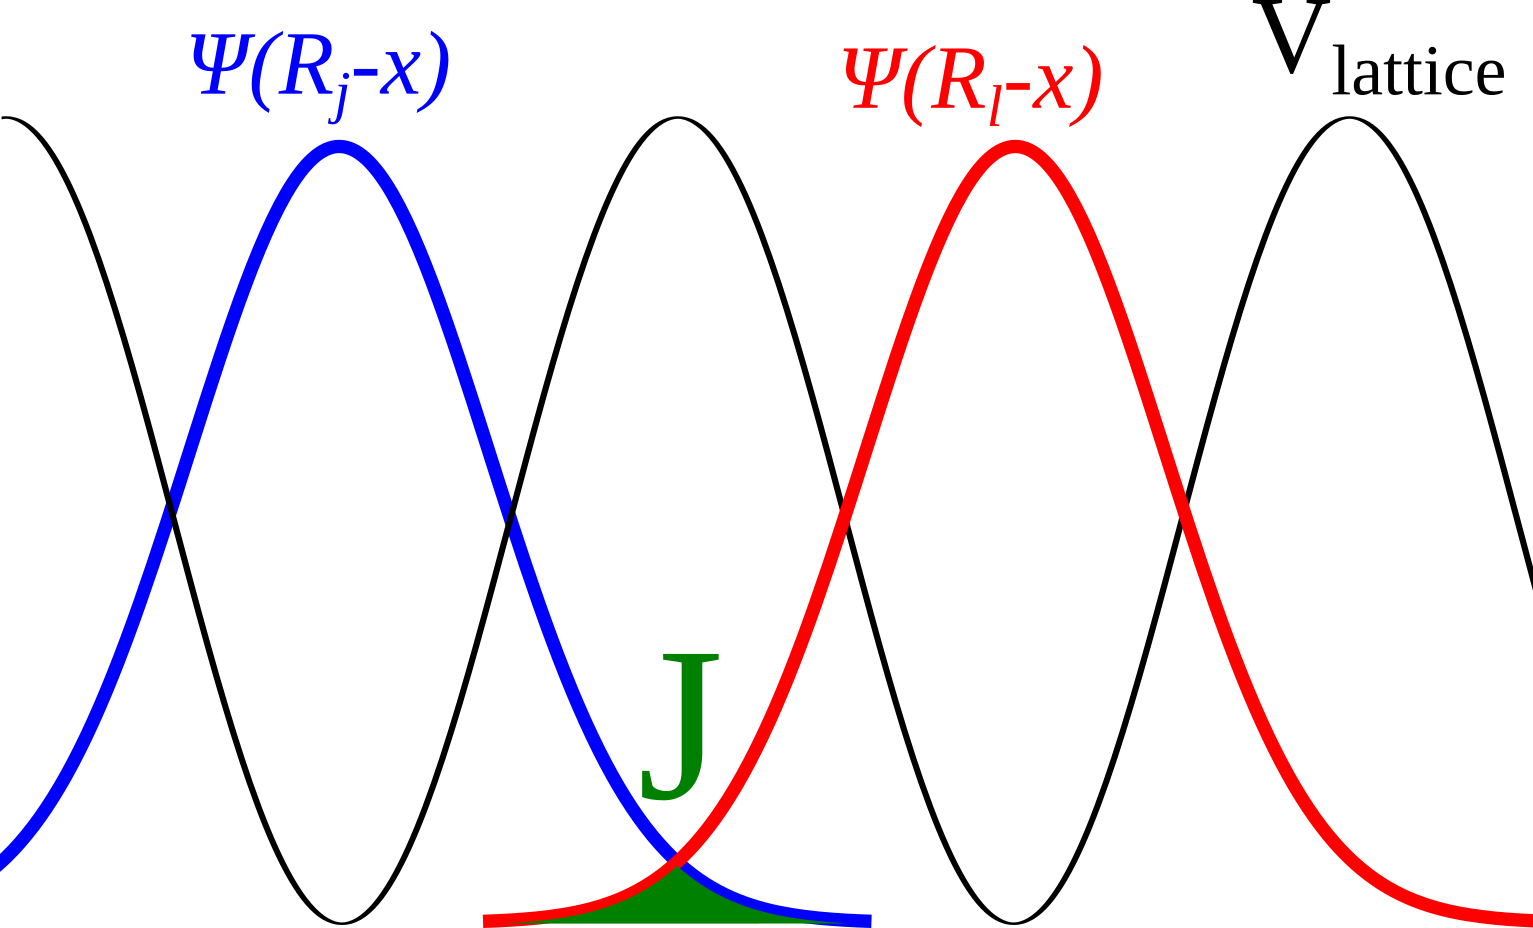
\includegraphics[width=0.8\textwidth]{J_overlap_drawing_smaller}
    \end{center}
    \caption{\label{fig:J_overlap_drawing}
             The strength of hopping $J$ is considered as the overlap of
             localised Wannier functions centred at neighbouring lattice sites.}
\end{figure}
This is not entirely accurate, as the Wannier states are orthonormal and so the
integral over their inner product is zero. More precisely, $J_{j,l}$ takes the
inner product between a Wannier state $\psi(R_{j} - x)$ and the state produced
by the action of $\hat{h}_1$ on the Wannier state $\psi(R_{l} - x)$, which does
not have to be zero. However, the depiction in figure \ref{fig:J_overlap_drawing}
can still be useful for developing an intuition for what $J$ is, since $J$
depends on the combination of the lattice depth (and width) and the kinetic
energy and so would the overlap of the spatial wave functions if they were not
orthonormal. It is also clear from the figure that computing overlap integrals
using wave functions on non-neighbouring sites does not add much accuracy to our
model, so we neglect these. For the hopping interactions that are permitted, we
assume that each has identical strength. This assumption allows us to write
\begin{equation}
    \hat{H}_{1}
    =
    \int{\hat{\psi}^{\dagger}(x)
         \bigg(
            \!\sum_{i}{-\frac{\hbar^{2}}{2m} \partial_{x_{i}}^{2}} +
            \sum_{j}{V_{\text{lattice}}(R_{j})}
         \bigg)
         \hat{\psi}(x) \,dx}
    =
    J \sum_{i}{(\hat{a}^\dagger_{i}\hat{a}_{i+1} + \text{h.c.})},
\end{equation}
where $\text{h.c.}$ denotes the hermitian conjugate. We can go through a similar
process for the contributions of the external potential and on-site interactions
between bosons. The external potential gives an on-site energy that can vary at
different locations in the lattice
\begin{equation}
    \hat{H}_{\text{ext}}
    =
    \int{\hat{\psi}^{\dagger}(x) V_{\text{ext}}(x) \hat{\psi}(x) \,dx}
    =
    \sum_{i}{\epsilon_{i} \hat{a}_{i}^{\dagger} \hat{a}_{i}}.
\end{equation}

The term for on-site interaction between bosons is a two-particle operator, thus
second quantisation requires integration between two sets of boson field
operators
\begin{equation}
    \hat{H}_{\text{int}} =
    \int{\hat{\psi}^{\dagger}(x) \hat{\psi}^{\dagger}(x)
          \frac{U_{0}}{2} \sum_{i,j}{\delta(x_{i}-x_{j})}
          \hat{\psi}(x) \hat{\psi}(x) dx
        }
    =
    \frac{U_{0}}{2}
    \sum_{i}
        {\hat{a}_{i}^{\dagger} \hat{a}_{i}^{\dagger} \hat{a}_{i} \hat{a}_{i}}
\end{equation}
Putting these terms together, we arrive at the Bose-Hubbard model described in
the next section.


\section{The Bose-Hubbard model}

The Hamiltonian for a weakly interacting BEC in a one-dimensional optical
lattice and subject to harmonic trapping potential is given by the sum of
$\hat{H}_{1}$, $\hat{H}_{\text{ext}}$ and $\hat{H}_{\text{int}}$:
\begin{equation}
    \hat{H}_{\text{1D}}
    =
    J \sum_{i}{(\hat{a}^\dagger_{i}\hat{a}_{i+1} + \text{h.c.})} +
    \frac{U_{0}}{2}
    \sum_{i}%
        {\hat{a}_{i}^{\dagger} \hat{a}_{i}^{\dagger} \hat{a}_{i} \hat{a}_{i}} +
    \sum_{i}%
        {\epsilon_{i} \hat{a}_{j}^{\dagger} \hat{a}_{j}},
\end{equation}
and is known as the Bose-Hubbard Hamiltonian. The $\epsilon_{i}$'s refer to
on-site energies at each lattice site due to the harmonic trap, and the middle
term gives an interaction energy when there is more than one particle on a
particular site. This project will look at scenarios where there is no external
harmonic potential which produces different on-site energies for different sites
(the uniform lattice potential remains, so $J$ is still defined as before). In
the absence of this external potential, the Hamiltonian in one dimension reduces
to
\begin{equation*}
    \hat{H}_{1D}
    =
    J \sum_{i}{(\hat{a}^\dagger_{i}\hat{a}_{i+1} + \text{h.c.})} +
    \frac{U_{0}}{2}
    \sum_{i}{\hat{a}^\dagger_{i} \hat{a}^\dagger_{i} \hat{a}_{i}\hat{a}_{i}}.
\end{equation*}

This project aims to explore the dynamics of both this one-dimensional system
and the two-dimensional version where we couple multiple chains of lattice
sites together. The system Hamiltonian in two dimensions is
\begin{equation}
    \hat{H}_{2D}
    =
    \left (
        J \sum_{i,j}{\hat{a}^{\dagger}_{i,j+1} \hat{a}_{i,j}} +
        J'\sum_{i,j}{\hat{a}^{\dagger}_{i,j} \hat{a}_{i+1,j}}
    \right) +
    \text{\text{h.c.}} +
    \frac{U_{0}}{2}
    \sum_{i}{\hat{a}^{\dagger}_{i}\hat{a}^{\dagger}_{i} \hat{a}_{i}\hat{a}_{i}},
\end{equation}
where the $i$ index denotes which chain is being referred to and the $j$ index
denotes how far along the chain a site is. $J'$ is another hopping parameter,
in this case characterising the hopping between sites on different chains.
\begin{figure}[H]
    \begin{center}
        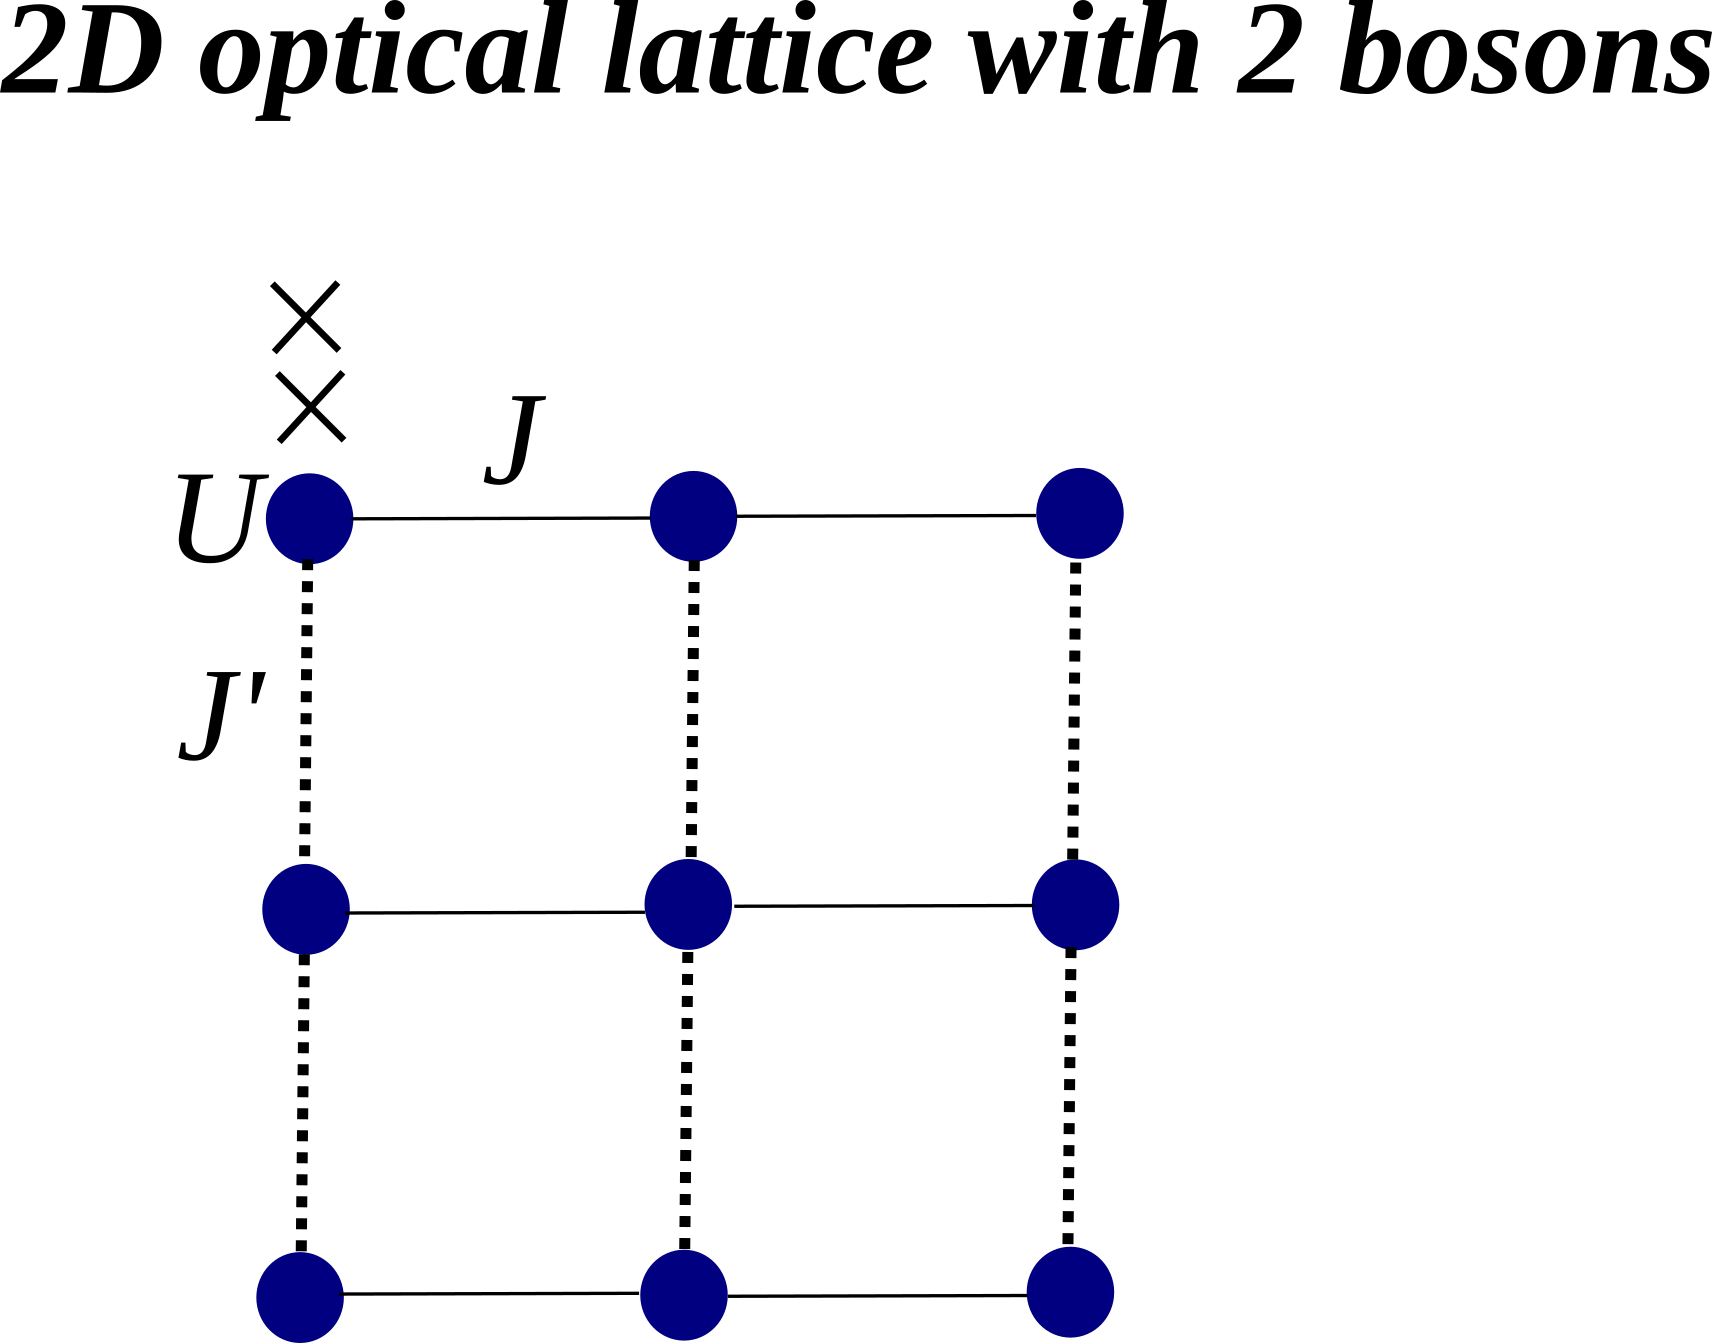
\includegraphics[width=8cm]{lattice_pic}
    \end{center}
    \caption{The blue circles here represent lattice sites and the crosses
             denote individual bosons. Hopping between any two neighbouring
             sites on the same chain is characterised by $J$, whereas hopping
             between chains is characterised by $J'$. A three by three lattice
             is shown here, but the system can be extended to arbitrary size.
            }
\end{figure}
We are interested in the time evolution of these systems as it relates to their
thermal behaviour.


\section{Thermalisation}

\subsection{Overview}

Thermalisation refers to a relaxation of a system to states where the values
of macroscopic quantities are stationary, universal with respect to widely
differing initial conditions, and predictable using statistical mechanics
\cite{Rigol2008}. We observe thermalisation in a wide variety of classical
systems, and there are strong theoretical reasons for anticipating this
thermalisation. However, many of these reasons don't apply when considering
quantum systems. The question of which, if any, quantum systems exhibit
thermalisation and how the thermal states can be characterised is of
considerable theoretical and experimental interest.

\subsection{Classical systems}

To see why thermalisation is common and even expected in many classical
systems, we need to understand the property of ergodicity and the impact of
chaotic dynamics on it. If you start an isolated system in a particular
configuration corresponding to a particular point in phase space, it can move
through that phase space along the constant-energy manifold. A system is
ergodic if the long-term time average of any single phase space trajectory
is equivalent to an ensemble average. 

Aside from a few rare examples that are usually emphasised in physics textbooks,
the equations of motion for most classical systems do not have simple analytic
solutions \cite{Jensen1992}. This means that we usually need to resort to
numerical methods to determine the evolution of these systems in time by solving
nonlinear partial differential equations. It is a well known fact about such
systems that they display an extreme sensitivity to the initial conditions, such
that the uncertainties or errors in the initial conditions can grow
exponentially as the system evolves in time, not merely as a result of numerical
approximations made but as an intrinsic property of the system. Our inability to
know the initial conditions of a real system presents an notoriously
challenging obstacle to long term predictions of these nonlinear systems, such
as the weather.

The nonlinearities present in chaotic systems drive them in seemingly irregular
motion. This allows the system to quickly and essentially uniformly explore the
constant-energy manifold irrespective of the initial conditions. This promotes
ergodicity, and thereby provides justification for the fundamental assumption
of statistical mechanics - all accessible microstates are equiprobable.
This combination of factors is what leads us to expect
our classical systems to thermalise.

\subsection{Quantum systems}

The time evolution of quantum mechanical systems is governed by the
Schr\"odinger equation, which is linear. This implies that the key ingredient
in producing dynamical chaos in classical systems, namely, the presence of
nonlinear equations of motion, is absent from quantum systems.

Without nonlinearities promoting exploration the phase space, it is
not obvious how one would justify applying the assumption of ergodicity to
quantum systems. Hence, it is unclear if, or when, we should expect quantum systems to
thermalise, or what statistical ensemble we could use to characterise the
relaxed states. One possible source of theoretical predictions is the
Eigenstate Thermalisation Hypothesis, (ETH) proposed independently by Deutsch
\cite{Deutsch1991} and Srednicki \cite{Srednicki1994}. If the necessary
conditions hold for the ETH to be applied, then it implies that the [eigenstates
of generic quantum Hamiltonians are “typical” in the sense that the statistical
properties of physical observables are the same as those predicted by the
microcanonical ensemble. The ETH implies that the expectation values
of such observables as well as their fluctuations in isolated quantum systems
far from equilibrium relax to (nearly) time-independent results that can be
described using traditional statistical mechanics ensembles.]\todo{part in
square brackets is copy pasted from \cite{DAlessio2016}}. Making predictions
about our system using the ETH would require considerable use of Random Matrix
Theory, which is beyond the scope of this dissertation but could form the basis
of future work.

\section{Integrable systems}

There are a number of classical, isolated systems that do not display
thermalisation. The main difference between these systems and those which
approach thermal equilibrium is the extent to which they are constrained
relative to the number of degrees of freedom that they possess. This observation
is formalised in the notion of integrability. A system is said to be integrable
if it has half as many independent integrals of motion (which are conserved)
as it has degrees of freedom. An integral of motion for a Hamiltonian is a
smooth function $I$ defined on an open subset of the phase space such that
$\dot{I}=0$ on solutions. \todo{reference handout Danny gave me, I can't see
anywhere where its from}So $I(x(t))=\text{constant}$, where $x(t)$ is the
solution of the equations of motion for a particular initial condition. If
$x_1(t)$ and $x_2(t)$ are solutions for different initial conditions, then in
most cases $I(x_1(t))\ne I(x_2(t))$. Integrability is a useful property, though
it is quite rare.

Theoretically, we can find exact solutions for the equations of motion for a
system if it is integrable, otherwise we cannot. In classical mechanics, the
idea of integrability is well-understood and neatly defined. The situation in
quantum mechanics is much more challenging. One reason for this is that
the Heisenberg uncertainty principle prevents us from applying the idea of
points in phase space with particular trajectories. However, a commonly 
used definition requires the presence of a large number of local operators (more
precisely, linear combinations of these operators) that commute with the 
Hamiltonian and each other and thus provide a set of conserved quantities. With 
respect to the systems that we are dealing with, it has been shown that a 
one-dimensional lattice chain of non-interacting bosons is an integrable 
system (with integrability given by the previously mentioned 
definition) \cite{Rigol2007}.

This is particularly interesting in light of the fact that the ETH is not 
satisfied for integrable systems. This may lead us to expect that we will 
not observe thermalisation in noninteracting one-dimensional systems, as it 
has recently been shown that the ETH must be satisfied for thermalisation to 
occur \cite{Palma2015} on the level of the eigenstates. Nonetheless, it has 
been argued \cite{DAlessio2016} that the existence of those conserved 
quantities does not preclude the thermalization of physical observables. 

The conserved quantities constrain the time evolution in such a way that not 
all of the constant-energy manifold is accessible. However, the system may 
still explore the reduced phase space ergodically. This idea has inspired 
the use of a generalised Gibbs ensemble (GGE), which includes a linear 
combination of the conserved quantities in the partition function, to predict 
the mean values of physical observables in whatever sort of equilibrium 
state that the integrable system relaxes into.

\section{Experimental studies}

\subsection{A quantum Newton's cradle}

Kinoshita et. al. investigated \cite{Kinoshita2006} the thermalisation of an
out-of-equilibrium one-dimensional Bose gas, which is a  nearly-integrable
system. They started with several thousand arrays of one-dimensional Bose gases,
each containing from $40$ to $250$ $^{87}$Rb atoms. The atoms were trapped by
combining a blue-detuned two-dimensional optical lattice, which provides tight 
transverse confinement, with a red-detuned crossed dipole
trap providing weak axial trapping. In order to create the non-equilibrium
momentum distributions, they then pulsed on a $3.2$ THz detuned one-dimensional
lattice, which depleted the zero momentum state and put the atoms in a
superposition momentum state of $\pm2\hbar k$. The two parts of the wavefunction
then oscillated out of phase with each other, colliding with each other twice
every full cycle and either reflecting off each other elastically or
transmitting straight through like a ``ghostly'' Newton's cradle (see figure 
\ref{fig:quantum_newtons_cradle}).
\begin{figure}[H]
    \begin{center}
        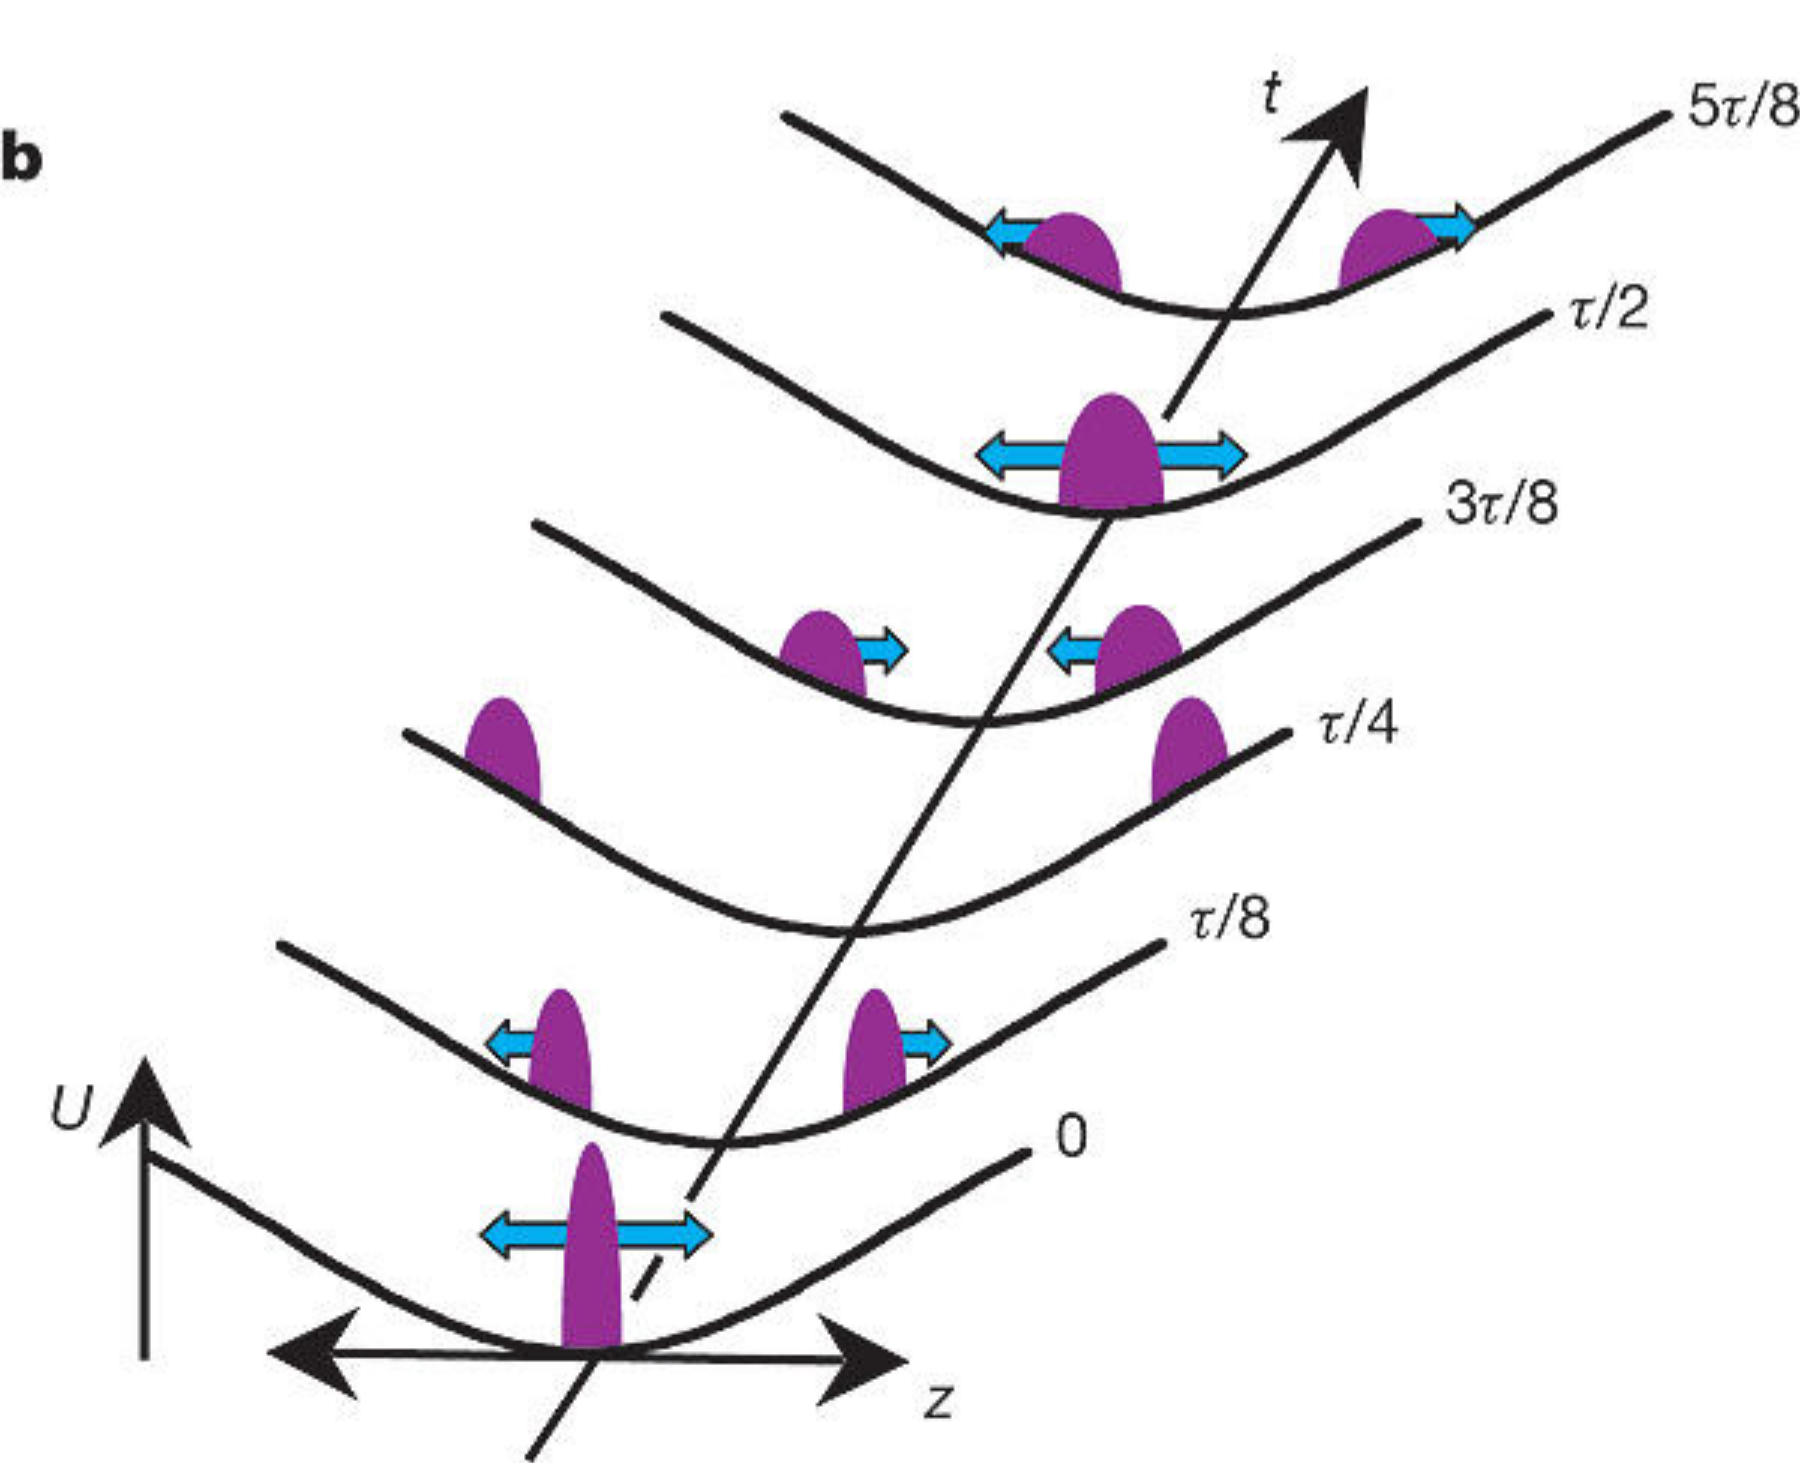
\includegraphics[width=8cm]{quantum_newtons_cradle}
    \end{center}
    \label{fig:quantum_newtons_cradle}
    \caption{Sketches at various times of two out of equilibrium clouds of atoms
             in a one-dimensional anharmonic trap. At time $t=0$ the atoms are
             put into a momentum superposition with $2\hbar k$ to the right and
             $2 \hbar k$ to the left. The two parts of the wave function
             oscillate out of phase with each other with a period $\tau$. Each
             atom collides with the opposite momentum group twice every full
             cycle, for instance, at $t=0$ and $t = \frac{\tau}{2}$. Figure is
             from reference \cite{Kinoshita2006}.}
\end{figure}
The weak anharmonicity of the trap caused the atoms to gradually dephase.
However, as can be seen from figure \ref{fig:dephased_momentum_distribution}, 
the momentum distribution after dephasing was not Gaussian (as one
would expect for a thermalised state), and did not noticeably
tend toward this Gaussian equilibrium distribution, even after thousands of 
collisions.
\begin{figure}[H]
    \begin{center}
    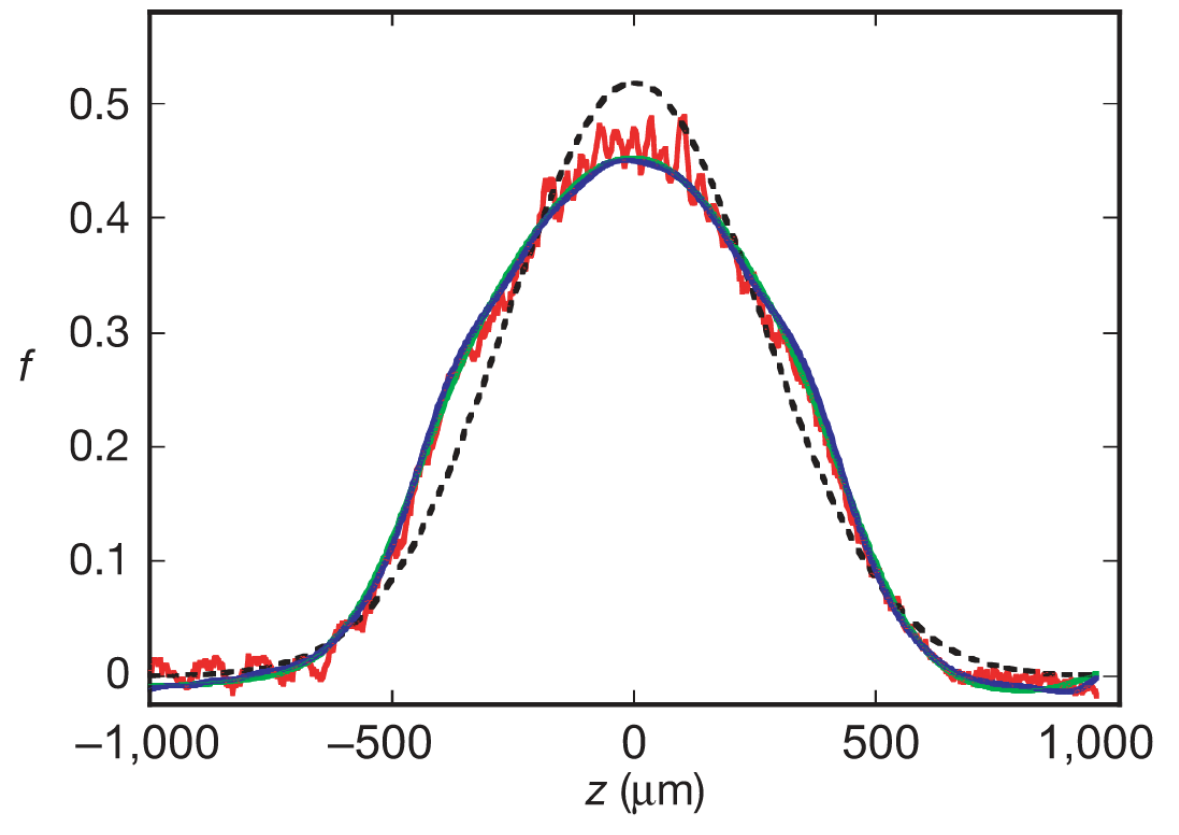
\includegraphics[width=1.0\textwidth]{dephased_momentum_distribution}
    \end{center}
    \caption{\label{fig:dephased_momentum_distribution}
             The blue and green curves in the above figure are projections from
             models that take into account loss and heating. The red line is the
             actual distribution observed. The dashed line is a Gaussian with
             the same number of atoms and r.m.s. width as the actual
             distribution.}
\end{figure}
To the extent that the actual distribution in figure
\ref{fig:dephased_momentum_distribution} conforms to the projected distribution
rather than to the Gaussian, the atoms have not thermalised. This absence of 
thermalisation extended from the Tonks--Girardeau regime, which has very
strong repulsive interactions between bosons so only pairwise collisions can
occur, to the intermediate coupling regime, where there can be three-
(or more) body collisions. This study represents a significant experimental 
breakthrough on the question of the time evolution of out-of-equilibrium 
one-dimensional Bose gases.

\subsection{Relaxation in an Integrable Many-Body Quantum System}

Inspired by the ``A Quantum Newton's Cradle'' study, investigations were made
into a completely integrable many-body quantum system, and the authors 
demonstrated strong agreement between their numerical data and the 
predictions generated using the generalised Gibbs ensemble. 
In this study the authors, Rigol et.
al \cite{Rigol2007}, started with a Hamiltonian for hard-core bosons with no
interactions on a one-dimensional lattice with $L$ lattice sites and 
periodic boundary conditions .
\begin{equation}
 \hat{H}=-J\sum_{i=1}^{L} (\hat{a}_{i}^{\dagger}\hat{a}_{i+1} + \text{h.c.})
\end{equation}
They then mapped their bosonic system to a free fermionic one using a
Jordan-Wigner transformation:
\begin{equation}
    \hat{H}
    =
    -J \sum_{i=1}^{L}{(\hat{c}_{i}^{\dagger}\hat{c}_{i+1} + \text{h.c.})}
\end{equation}
Here $\hat{c}_{i}^{\dagger}$ and $\hat{c}_{i+1}$ are fermionic creation and
annihilation operators. The integrals of motion were the fermionic
quasi-momentum distribution operators, and the system thus must be
integrable because there are as many of these operators as they had lattice
sites. They have numerically investigated the time evolution of this system and
found it to undergo relaxation to an equilibrium state. The quasi-momentum 
distribution of this equilibrium state was shown to have excellent
agreement (see figure \ref{fig:GGEquasimomentum}) with the predictions of a 
generalised Gibbs ensemble, in which the partition function is extended to 
include all of the integrals of motion.
\begin{figure}[H]
    \begin{center}
        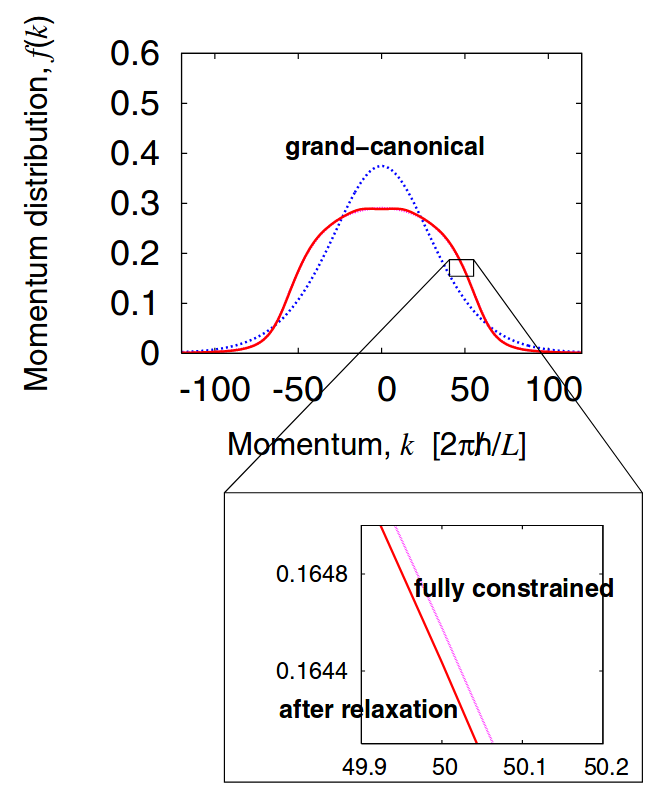
\includegraphics[width=8cm]{grand_canonical_vs_GGE}
    \end{center}
    \caption{\label{fig:GGEquasimomentum}Equilibrium (quasi-)momentum distribution after relaxation in
             comparison with the predictions of the grand-canonical and of the
             fully constrained thermodynamic ensembles. The prediction of the
             fully constrained  ensemble is virtually indistinct from the
             results of the dynamical simulation. Image taken from
             \cite{Rigol2007}.}
\end{figure}
They further showed that their generalised equilibrium state carries more memory
of the initial conditions than the usual thermodynamic one, which is consistent
with their system not satisfying the ETH because it is integrable.
% \begin{figure}[H]
%     \begin{center}
%         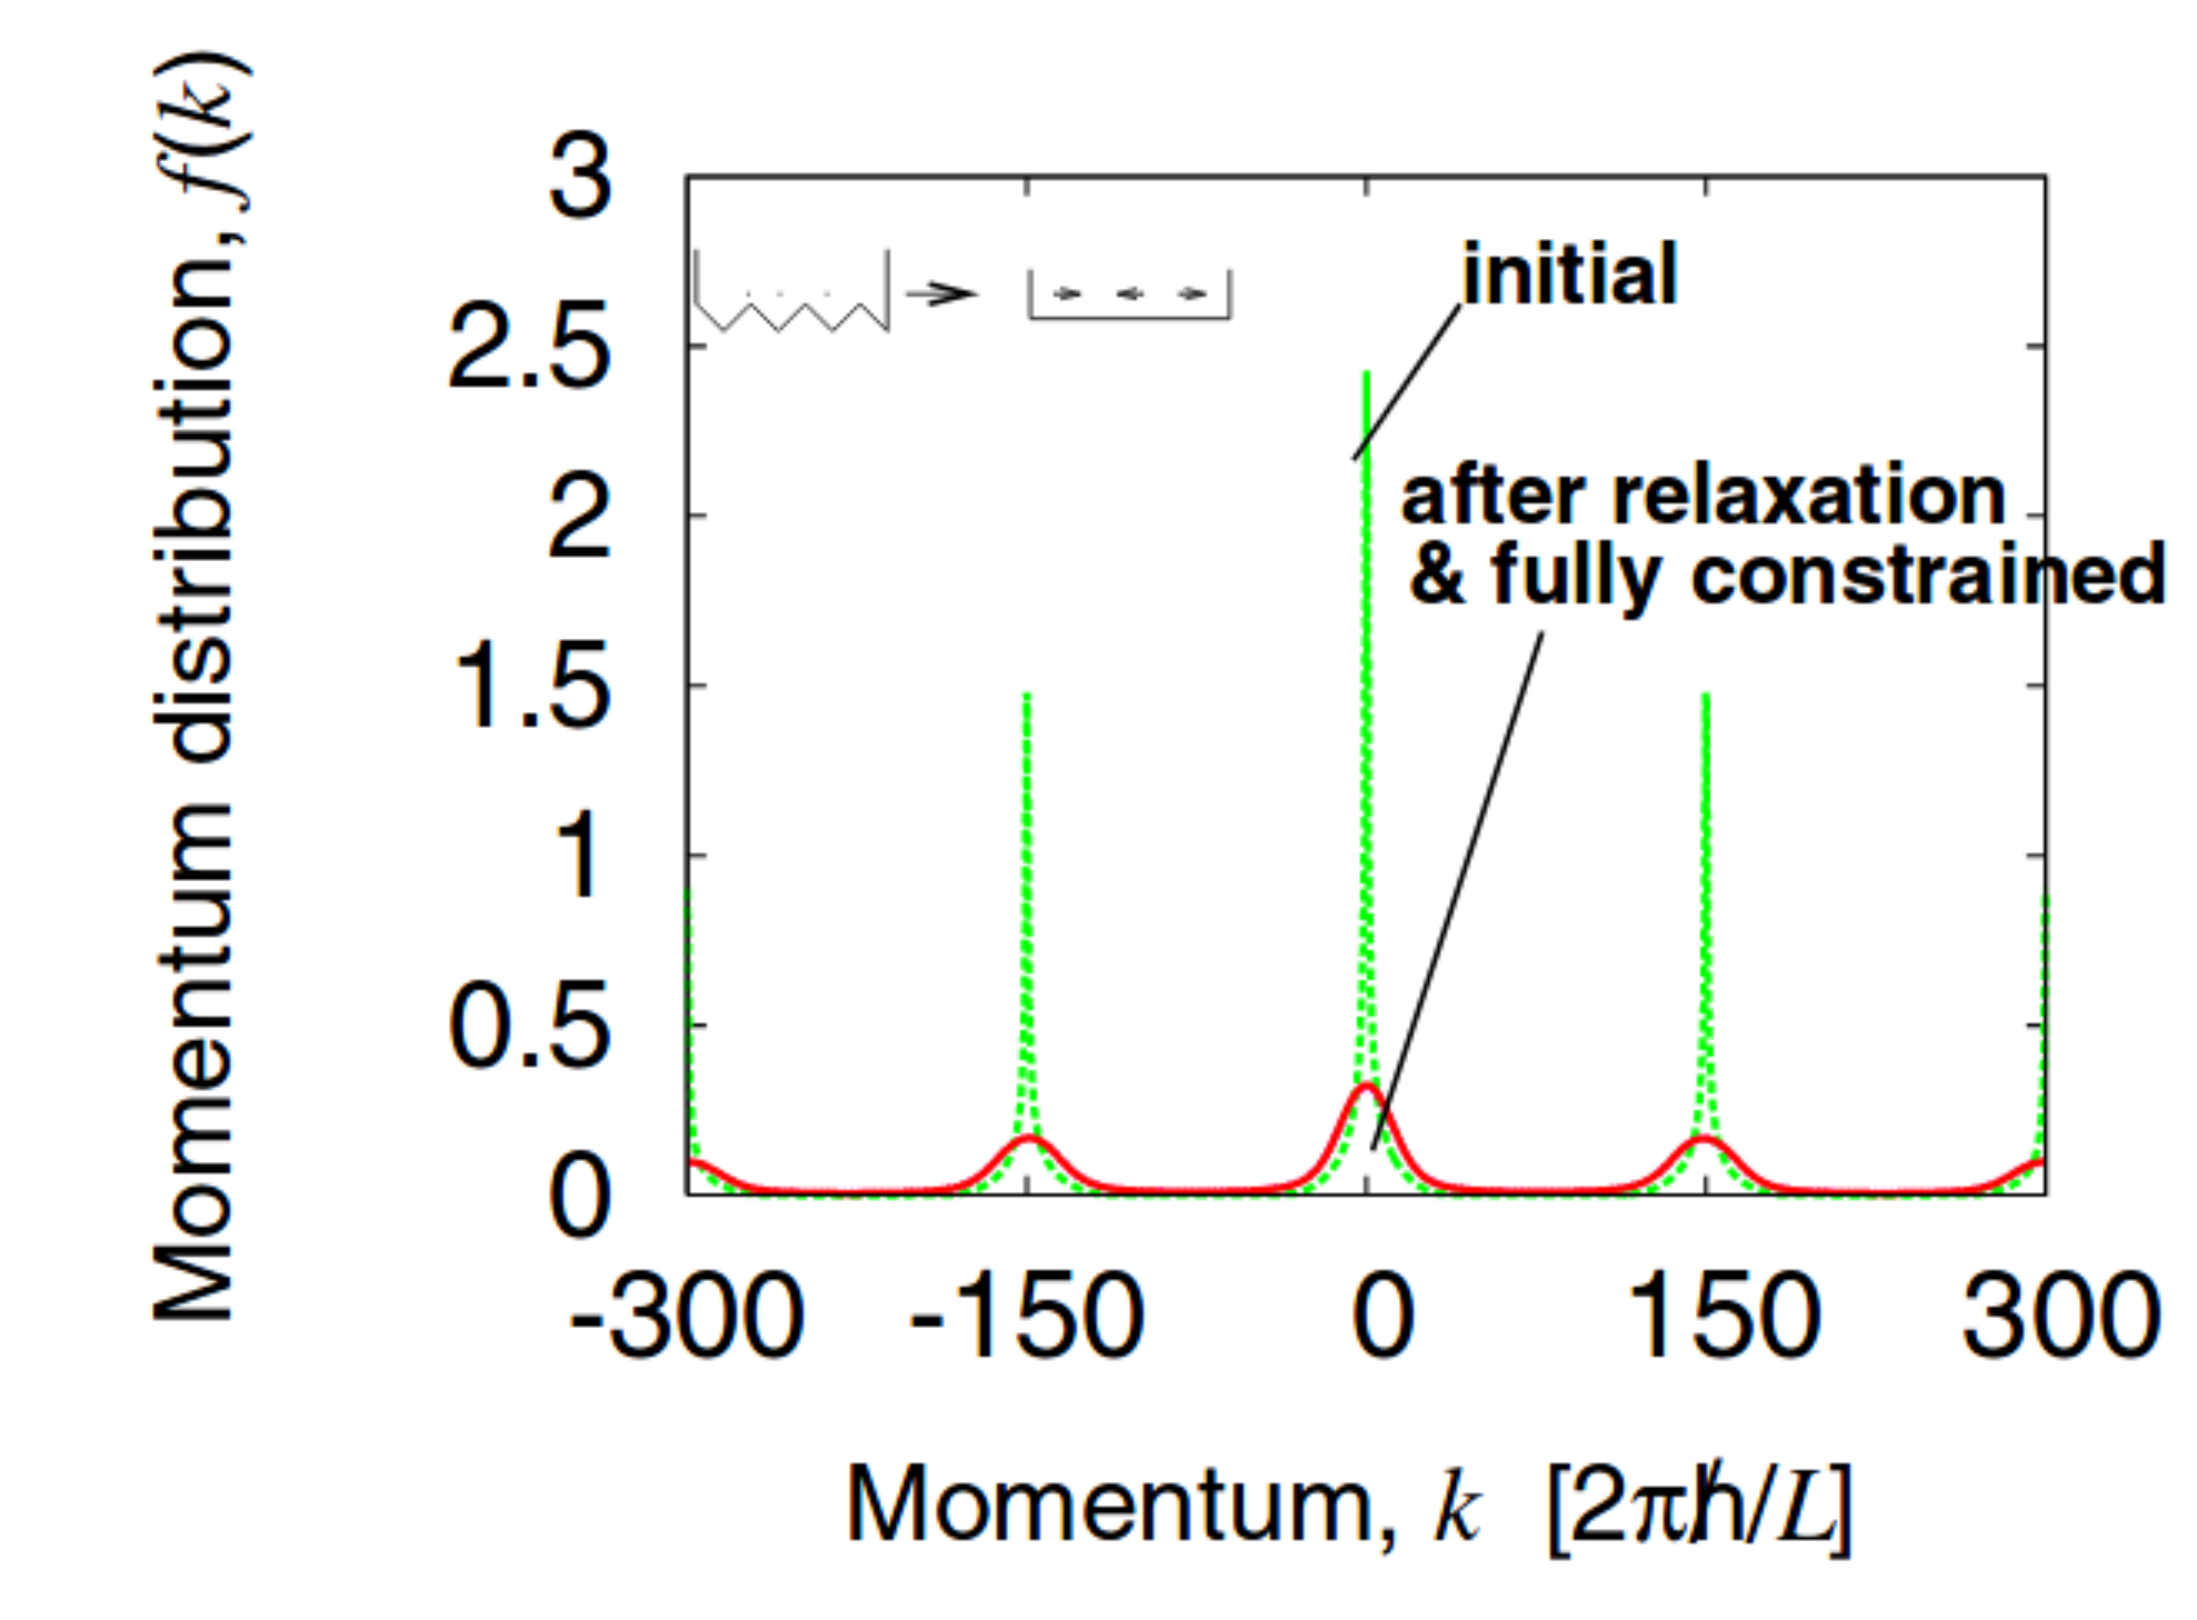
\includegraphics[width=8cm]{after_relaxation_rigol}
%     \end{center}
%     \caption{The actual quasi-momentum distribution after relaxation versus
%              predictions of the generalised Gibbs ensemble and the grand
%              canonical ensemble. Image taken from \cite{Rigol2007}.}
% \end{figure}
% The momentum peaks remain clear and distinct during the whole duration  of
% propagation; $t_{\text{fin}} = 3000 \hbar/J$.


\section{System size and analyticity}

Whilst the main focus of this project is on smaller lattices with few particles,
it is of interest to investigate larger system sizes (necessarily by approximate
methods) to see how much of the qualitative behaviour of the small systems is
preserved in the larger ones.

\subsection{Small systems}

We can decompose any time evolved state $\ket{\psi(t)}$ of our system in terms
of its state at $t=0$, $\ket{\psi(0)}$, and the energy eigenvectors $\ket{E_n}$
(see section \ref{revival} for details):
\begin{equation}
    \label{eq:SmallSystems_PsiTimeEvolution}
    \ket{\psi(t)} = \sum_{j}{e^{i E_{j}t} \ket{E_{j}} \braket{E_{j}|\psi(0)}}.
\end{equation}
Calculating $\ket{\psi(t)}$ from the above formula requires that we diagonalise
the Hamiltonian and find its energy eigenvectors and eigenvalues. This is easy
for small systems, in particular those that have only a single particle on them.
This method has the significant advantage of being ``analytic'', at least up to
the precision of the values stored for the eigenvalues and eigenvectors. All
instances of $\ket{\psi(t)}$ are calculated from the initial state
$\ket{\psi(0)}$, so the value we calculate for $\ket{\psi(t)}$ is independent of
the time-step between each instance of $\ket{\psi(t)}$ that we calculate. This
has the further advantage that in a numerical algorithm we need not concern
ourselves with drifting of the norm. However, as the number of lattice sites and
particles in the system increases, the time required to apply this method
increases dramatically. This is because the dimensionality $\mathcal{D}$ of the
system grows according to
\begin{equation}
    \label{dimensionality_exact}
    \mathcal{D} = \frac{(N + P - 1)!}{P! (N-1)!},
\end{equation}
where $N$ is the number of lattice sites and $P$ is the number of particles on
the lattice. Unsurprisingly, this is the same as the number of possible pure
number states (since these form an orthonormal basis), and so the formula
deduced is just the formula for the number of ways to arrange $P$ objects into
$N$ containers that is familiar from elementary statistical mechanics.
The Hamiltonian can be represented in the basis of energy eigenvalues as a
$\mathcal{D} \times \mathcal{D}$ square matrix. However diagonalising this
matrix, determining its energy eigenvalues and then evolving the system
according to equation \eqref{eq:SmallSystems_PsiTimeEvolution} quickly becomes
impractical for systems with large numbers of particles and lattice sites. 

We can use another familiar tool from elementary statistical mechanics 
--Stirling's approximation-- to clarify the rate of growth of the 
dimensionality of the system. Stirling's approximation \cite{Schroeder2007} is
\begin{equation}
    N! \approx N^{N} e^{-N} \sqrt{2 \pi N}.
\end{equation}
All of the following assumptions (including Stirling's approximation) are
valid only for large $N$.
\begin{equation*}
    \mathcal{D} = \frac{(N + P - 1)!}{P! (N-1)!}
    \approx
    \frac{(N + P)!}{P! N!}.
\end{equation*}
Now applying Stirling's approximation to each factorial:
\begin{equation*}
    \mathcal{D}
    \approx
    \frac{(P + N)^{P+N} e^{-(P + N)} \sqrt{2 \pi (P+N)}}
         {P^{P} e^{-P} N^{N} e^{-N} 2 \pi \sqrt{PN}}
    =
    \frac{(P + N)^{P+N} \sqrt{2 \pi (P+N)}}
         {P^{P} N^{N} 2\pi \sqrt{PN}}.
\end{equation*}
The exponentials are much more significant than the multiplicative factors, so
we have
\begin{equation*}
    \mathcal{D} \approx \frac{(P + N)^{P+N}}{P^P N^N}.
\end{equation*}
In order to get a more concrete idea of how quickly the dimensionality of a
typical system would grow, consider the case where we have roughly one boson
per lattice site ($N \approx P$). In this case,
\begin{equation*}
    \mathcal{D} \approx \frac{(2P)^{2P}}{P^{P} P^{P}} = 2^{2P} = 4^{P}.
\end{equation*}
This means that when we increase the size of the system by one lattice site with
one boson on it, the dimensionality roughly quadruples. In light of this
exponential increase in dimensionality for large systems, a different approach
to time evolution is required. We have chosen to use a Gross-Pitaevskii equation
to overcome or at least control the curse of dimensionality of the system. Doing
this forces us to take an iterative approach to time evolution rather than an
analytic one. A Runge-Kutta-Feldberg algorithm \cite{Burden2005} was written for
this purpose.


\subsection{The Gross-Pitaevskii Equation}

The Gross-Pitaevskii Equation (GPE) is a classical mean-field equation for
describing Bose-Einstein condensates (BECs) in the zero-temperature limit 
\cite{Pitaevskii2003}. The validity of some of the assumptions that we make 
in this mean-field method will rely on there being a large number of particles. 
This is something that we cannot explore with our many-body treatment. When 
second quantising our Hamiltonian earlier, in equation 
(\ref{field_operators_wannier}) we decomposed
the field operators into linear combinations of single-particle Wannier position
states. However, it is possible to decompose the field operators into any
complete single-particle basis. If we chose the single particle energy basis
$\lbrace \phi_{i} \rbrace$, then we get
\begin{equation}
    \hat{\Psi}(\mathbf{r})
    =
    \sum_{i=0}^{\infty}{\hat{a}_i\phi_{i}(\mathbf{r})}
    =
    \hat{a}_{0} \phi_{0}(\mathbf{r}) +
    \sum_{i=1}^{\infty}{\hat{a}_i\phi_{i}(\mathbf{r})}.
\end{equation}
Since the GPE is a tool for investigating near-zero temperature BECs (very low
energy systems), we now assume that the occupancy of energy modes other than
the ground modes is negligible, i.e.,
\begin{equation}
    \hat{\Psi}(\mathbf{r}) = \hat{a}_{0} \phi_{0}(\mathbf{r}).
\end{equation}
Next we note that when there are a large number of particles in the ground state
$\ket{N_{0}}$ then the action of the creation and destruction operators on the
ground state approximately commute:
\begin{equation}
    \hat{a}_{0} \hat{a}^{\dagger}_{0} \ket{N_{0}}
    =
    N_{0} \sqrt{1+1/N_{0}} \ket{N_{0}}
    \approx
    N_{0} \ket{N_{0}}
    =
    \hat{a}^{\dagger}_{0} \hat{a}_{0} \ket{N_{0}}
\end{equation}
It is this property of commutation that leads us to replace the creation and
annihilation operators by $\sqrt{N_{0}}$, which is much simpler algebraically 
and allows us to approximate the field operator $\hat{\Psi}(\mathbf{r})$ with 
a wave function
\begin{equation}
    \hat{\Psi}(\mathbf{r})
    =
    \hat{a}_{0} \phi_{0}(\mathbf{r}) \approx \sqrt{N_{0}} \phi_{0}(\mathbf{r})
    =
    \Psi_{0}(\mathbf{r}).
\end{equation}

If we do this, then the equation of motion for the field operator in the 
Heisenberg picture becomes an equation for the time evolution of the 
condensate wavefunction (The time-dependent Gross-Pitaevskii equation)

\begin{equation}
 i\hbar \frac{\partial\Psi_{0}(\mathbf{r},t)}{\partial t}
 = 
 \left( 
 \frac{-\hbar^2\nabla^2}{2m}
 +
 V_{\text{lattice}}(\mathbf{r})
 +
 U_0 |\Psi_{0}(\mathbf{r},t)|^2 
 \right)
 \Psi_{0}(\mathbf{r},t)   .
\end{equation}
It is worth noting that this equation is normalised to $1$, and makes no 
reference to particle number. This will become relevant later, when we want
to compare many-body simulations and GPE simulations with identical 
interparticle interaction strengths. 
\subsection{Runge-Kutta-Feldberg Method}

The nonlinear term in the GPE prevents us from being able to represent the
Hamiltonian in matrix form. Hence we cannot find the eigenvectors and
eigenvalues of the system directly, which prevents us from using the ``analytic''
approach to time evolution that we used for smaller system sizes. One method
that we could use in its pace is to simply expand the time evolution operator
$e^{-i \hat{H} t}$ in a Neumann series of the operator $\hat{H}$, truncated at
an appropriate order, i.e.,
\begin{equation}
    \ket{\psi(t)}
    =
    e^{-i\hat{H}t}\ket{\psi(0)}
    =
    \left (
        1 + (-i \hat{H} t) + \frac{1}{2}(-i \hat{H} t)^{2} +
        \frac{1}{6}(-i \hat{H} t)^{3} + \dots
    \right)
    \ket{\psi(0)}.
\end{equation}
When we are working with systems in which $U_{0} \neq 0$, the nonlinearity that
is present quickly causes inaccuracies in any low-order ($\leq3$) method.
The deterioration of numerical accuracy can be observed by calculating the norm
of $\ket{\psi(t)}$ at each timestep. It quickly grows significantly greater than
1. Here we need to compromise as using a higher-order method is slow, due to the
computation time required to calculate the powers of $hat{H}$ at
each timestep.

A standard Runge-Kutta method speeds up the calculation by avoiding calculating
these terms while retaining high-order truncation error. One of the most
frequently used Runge-Kutta methods is a fourth order method, which has
truncation error of $\mathcal{O}(h^4)$, where $h$ is the size of the timestep.

For a given differential equation
\begin{equation}
    y' = f(t,y)
\end{equation}
with initial condition $y(t=0) = \alpha$, we can approximate the value of $y$ at
$N$ successive times (each separated by timestep $h$) by $w$, where
\begin{align*}
    w_{0}   &= \alpha
    \\
    k_{1}   &= hf(t_{i}, w_{i})
    \\
    k_{2}   &= hf \left( t_{i} + \frac{h}{2}, w_{i} + \frac{1}{2} k_{1} \right)
    \\
    k_{3}   &= hf \left( t_{i} + \frac{h}{2}, w_i+\frac{1}{2} k_{2} \right)
    \\
    k_{4}   &= hf (t_{i+1}, w_{i+k_{3}})
    \\
    w_{i+1} &= w_{i} + \frac{1}{6}(k_{1} + 2 k_{2} + 2 k_{3} + k_{4})
\end{align*}
for each $i = 0$, 1, \dots, $N-1$.

Even when using this method, we are concerned about the effect of the nonlinear
term on error. Hence we adopt a more sophisticated, adaptive algorithm, the
Runge-Kutta-Feldberg method. This method incorporates an estimate of the
truncation error and adapts the step size as it goes to ensure that the error
stays below a certain tolerance set by the user.

Specifically, it uses a Runge-Kutta method of order five to estimate the
local error in a Runge-Kutta method of order four. If the estimated error
is greater than the tolerance, then the timestep is reduced and the error is
estimated again. The interested reader may refer to chapter $5$ of
\emph{Numerical Analysis} by R. Burden and J. Faires \cite{Burden2005} for the
further details of the algorithm used.
\newpage


\section{Results}

\section{Revival \label{revival}}

In a subset of the integrable systems considered, we observed regular instances
in which the system would return to the state in which it was initially
prepared (it ``revives''). To see why we might expect to see revival in
some cases, consider the initial state of the system $\ket{\psi(0)}$, which
evolves in time according to
\begin{equation}
    \ket{\psi(t)} = e^{i \hat{H} t} \ket{\psi(0)},
\end{equation}
where --for sake of brevity and transparency-- the constant $\hbar^{-1}$ has
been incorporated into the time scale. Now noting that we can use the
completeness relation for the energy eigenstates to expand the initial state in
the energy basis one obtains
\begin{align}
\label{time_evolution}
 \ket{\psi(t)} &= e^{i\hat{H}t}\sum_j\ket{E_j}\braket{E_j|\psi(0)}  \nonumber \\
               &= \sum_je^{i\hat{H}t}\ket{E_j}\braket{E_j|\psi(0)}  \nonumber \\
               &= \sum_je^{iE_{j}t}\ket{E_j}\braket{E_j|\psi(0)}    \nonumber \\
               &= \sum_j c_{j}e^{iE_{j}t}\ket{E_j}.
\end{align}
From here it can be seen that the only time dependence appears in the complex
exponentials, each of which is $2 \pi$-periodic. If we can find some common time
$t^{\ast}$ such that $E_{j} t^{\ast} = 2 \pi k_{j}$, where $k_{j} \in\mathbb{Z}$
for all $j$, we will recover the initial state exactly, i.e.,
$\ket{\psi(t^{\ast})} = \ket{\psi(0)}$. The next section describes the
conditions necessary for the existence of the revival time.


\subsection{Exact revival}

We observe an exact and regular revival in precisely the cases in which the
eigenvalues are mutually rational, i.e., they are either all rational, or are
all rational when divided by the same irrational number.
\begin{definition}[Mutually rational set]
    We say that a set of eigenvalues are mutually rational if they are all
    rational when divided by a common real number.
\end{definition}
For example, the set of hypothetical eigenvalues $\lbrace 0, \sqrt{2}, 2
\sqrt{2}, \frac{3 \sqrt{2}}{10} \rbrace$ is mutually rational, whereas $\lbrace
0, \sqrt{2}, \sqrt{3}\rbrace$ is not. In the case of mutually rational
eigenvalues, we can write $E_{j} = \frac{p_{j}}{q_{j}}$, where $p_{j}$, $q_{j}
\in \mathbb{Z}$. The revival time is then given by
\begin{equation}
    \label{revival_time_formula}
    t^{\ast} = \frac{2 \pi Q_{\text{LCM}}}{P_{\text{HCF}}},
\end{equation}
where $Q_{\text{LCM}}$ is the lowest common multiple of $\lbrace q_{j} \rbrace$
and $P_{\text{HCF}}$ is the highest common factor of the $\lbrace p_{j} \rbrace$.

We are yet to find any systems with nonzero interparticle interaction that have
mutually rational eigenvalues. In one dimension, the only systems that we have
found that meet the criterion of mutually irrational eigenvalues are those with
fewer than 4 lattice sites. In two dimensions, the only systems that exhibit
revival have three or fewer chains and three or fewer lattice sites on each
chain (see section \ref{2Dsystems}).

To demonstrate this exact revival, consider a one-dimensional lattice with three
sites with a single boson and hopping constant $J$. The Hamiltonian for this
system is
\begin{equation}
    \hat{H}_{3\times1}
    =
    \begin{pmatrix}
         0 & -J &  0 \\
        -J &  0 & -J \\
         0 & -J &  0
    \end{pmatrix}.
\end{equation}
Diagonalising this matrix yields the eigenvalues $\lbrace -\sqrt{2}J, 0,
\sqrt{2} J \rbrace$. These are mutually rational (if we divide them all by
$\sqrt{2}J$ they are all rational). If we rescale the energies by $\sqrt{2}J$ by
absorbing that factor into the time scale, then we get eigenvalues $\{-1,0,1\}$.
We can see from the graph of the simulation below that this matches up with a
return to the initial state at times that are multiples of $2\pi$.
\begin{figure}[H]
    \centering
    \begin{gnuplot}[terminal=cairolatex, terminaloptions={lw 2}, scale=0.95]
        set xlabel "$\\displaystyle \\frac{t}{\\sqrt{2}J}$"
        set ylabel "$\\langle n_{1} \\rangle$"
        plot "./Data/20170912T164043_evolution_n.dat" u 1:4 w l lc 1 notitle
     \end{gnuplot}
     \vspace*{-5mm}
     \label{fig:3by1_noninteract_revival}
     \caption{Revival for a system with 3 lattice sites and a single boson.}
\end{figure}

The reason that there appear to be several revivals that our method ``misses''
is that states with different phases in the coefficients of the eigenvectors
can also produce $\langle n_{1} \rangle = 1$, whereas the revival time that is
calculated in our method corresponds to exact revival of the initial
wave function and not $\langle n_{1} \rangle \sim \norm{\psi(t)}^{2}$.


\subsection{Approximate revival}

The range of systems for which the eigenvalues are mutually rational is a small
one. All systems which have nonzero interparticle interactions have mutually
irrational eigenvalues. One of the most interesting results so far is that
even in the one-dimensional single particle case, if there are more than
three lattice sites, the eigenvalues will be irrational. We can demonstrate this
by considering a single chain of five sites with one boson. The Hamiltonian for
this system is
\begin{equation}
    \hat{H}_{5\times1}
    =
    \begin{pmatrix}
         0 & -J &  0 &  0 &  0 \\
        -J &  0 & -J &  0 &  0 \\
         0 & -J &  0 & -J &  0 \\
         0 &  0 & -J &  0 & -J \\
         0 &  0 &  0 & -J &  0
    \end{pmatrix}.
\end{equation}
The eigenvalues of this system are $\lbrace -\sqrt{3}J, -J, 0, J, \sqrt{3}J
\rbrace$. These are clearly not mutually rational, so we cannot find an exact
revival time for this system, despite the fact that it is fully integrable
\cite{Rigol2007}.

Note that the eigenvalues of a system with $4$ lattice sites are also mutually
irrational as they are
\begin{equation*}
    \frac{J}{2}\,
    \left \lbrace
        -1 - \sqrt{5}, 1 + \sqrt{5}, 1 - \sqrt{5}, -1 + \sqrt{5}
    \right \rbrace
\end{equation*}
but those for a system of 5 lattice sites are more convenient to work with.

Running a simulation of this system of $5$ lattice sites where we start a single
boson off on the first site, we find that the probability of finding the boson
on the first site never quite reaches unity again.
\begin{figure}[H]
    \centering
    \begin{gnuplot}[terminal=cairolatex, terminaloptions={lw 2}, scale=0.95]
        set xlabel "$\\displaystyle \\frac{t}{J}$"
        set ylabel "$\\langle n_{1} \\rangle$"
        plot "./Data/5by1_T1e4.dat" u 1:6 w l lc 1 notitle
     \end{gnuplot}
     \vspace*{-5mm}
     \caption{Absence of exact revival for a system with 5 lattice sites and a
              single boson.}
\end{figure}

Judging the figure above by eye, it may appear that we have exact revival, but
this is not actually the case. If we look at how long it takes for the system to
get within $\epsilon$ of its initial state (i.e. $\norm{\ket{\psi(t)} -
\ket{\psi(0)}} < \epsilon$) we get the graph below. Note that $t^{\ast}$ denotes
the time at which the system got within a particular value of $\epsilon$ of the
initial state the first time after $t=0$.
\begin{figure}[H]
    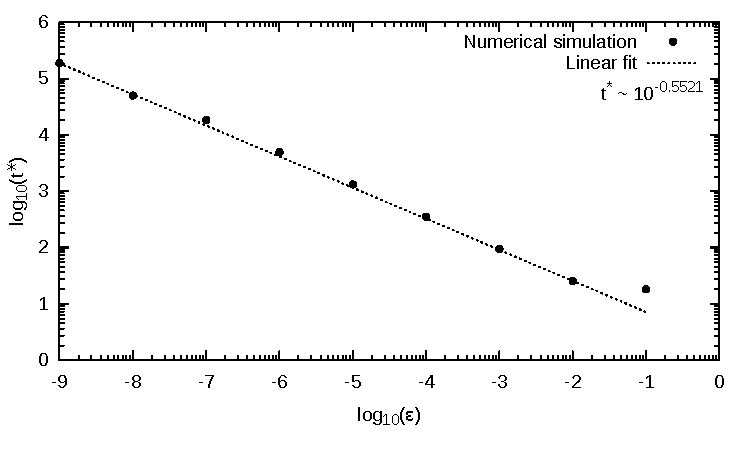
\includegraphics[width=1.0\textwidth]{recurrence_times}
    \centering
    \label{1Drecurrencetimes}
\end{figure}
While we see that the system does appear to get arbitrarily close to revival,
but it can take arbitrarily long to do so. This result can be explained in terms
of the Poincar{\'e} recurrence theorem.


\subsection{The Poincar\'e Recurrence Theorem}

In 1890, Henri Poincar{\'e} proved \cite{Poincare1890, Poincare2017} the
following theorem for classical mechanics:
\begin{quote}
    Any phase-space configuration $(q, p)$ of a system enclosed in a finite
    volume will be repeated as accurately as one wishes after a finite (be it
    possibly very long) interval of time.
\end{quote}
This theorem was extended to quantum systems in 1956 by P. Bocchieri and A.
Loinger \cite{Bocchieri1957}, where they gave a slightly different form:
\begin{theorem*}[Quantum recurrence]
    Let us consider a system with discrete energy eigenvalues $E_{n}$; if
    $\Psi(t_{0})$ is its state vector in the Schr{\"o}dinger picture at the time
    $t_{0}$ and $\epsilon$ is any positive number, at least one time $t^{\ast}$
    will exist such that the norm $\norm{\Psi(t^{\ast}) - \Psi(t_{0})}$ of the
    vector $\Psi(t^{\ast}) - \Psi(t_{0})$ is smaller than $\epsilon$.
\end{theorem*}
\begin{proof}
    The proof presented by Bocchieri and Loinger shows the theorem to be true
    for an infinite-dimensional system. In this dissertation, we investigate
    only finite-dimensional systems, and a simpler version of the proof can be
    constructed. We first show that there is a time $t^{\ast}$ at which
    $\norm{\ket{\psi(t^{\ast})} - \ket{\psi(t_{0})}}^{2} < 2 \epsilon'$ for any
    $\epsilon' > 0$ and then extend this to $\norm{\ket{\psi(t^{\ast})} -
    \ket{\psi(t_{0})}} < \epsilon$. Note that in the following we will introduce
    the notation $\tau=t^{\ast} - t_{0}$ and $\alpha^{2}(t^{\ast}) = \norm{
    \ket{\psi(t^{\ast})} - \ket{\psi(t_{0})}}^{2}$.

    Let us establish an upper bound for $\alpha(t^{\ast})$. Since $\alpha^{2}$
    is the square of the norm, we can write it as a scalar product of
    $\ket{\psi(t^{\ast})} - \ket{\psi(t_{0})}$ with itself, and also expand
    each wavefunctions in the basis of energy eigenfunctions.
    \begin{align*}
        \alpha^2(t^{\ast})
        &=
        \left ( \bra{\psi(t^{\ast})} - \bra{\psi(t_{0})} \right )
        \left ( \ket{\psi(t^{\ast})} - \ket{\psi(t_{0})} \right )
        \\
        &=
        2 - \braket{\psi(t^{\ast})|\psi(t_{0})} -
            \braket{\psi(t_{0})|\psi(t^{\ast})}
        \\
        &=
        2 -
        \sum_{j,n=1}^{\mathcal{D}}
            {c_{n}^{\ast} c_{j} e^{i E_{n} t^{\ast}} e^{-i E_{j} t_{0}}
             \braket{E_n|E_j}
            }
        -
        \sum_{j,n=1}^{\mathcal{D}}
            {c_{j}^{\ast} c_{n} e^{i E_{j} t_{0}} e^{-i E_{n} t^{\ast}}
             \braket{E_j|E_n}
            }.
    \end{align*}
    Since the energy eigenfunctions are orthonormal, $\braket{E_j|E_n} =
    \delta_{ij}$, the right hand side simplifies to
    \begin{equation*}
        \alpha^2(t^{\ast})
        =
        2 -
        \sum_{n=1}^{\mathcal{D}}{\abs{c_{n}}^{2} e^{i E_{n} (t^{\ast} - t_{0})}}
        -
        \sum_{n=1}^{\mathcal{D}}{|c_n|^2 e^{-iE_{n}(t^{\ast}-t_{0})}}.
     \end{equation*}
     Furthermore due to the totality of the energy basis the $\ell_{2}$ norm of
     the expansion coefficients is unity, i.e., $\sum_{n=1}^{\mathcal{D}}%
     {\abs{c_{n}}^{2} = 1}$, thus
    \begin{equation*}
        \alpha^2(t^{\ast})
        =
        2
        \sum_{n=1}^{\mathcal{D}}
            {\abs{c_{n}}^{2} \left ( 1 - \cos{\!(E_{n} \tau)} \right)}
        \leq
        2
        \sum_{n=1}^{\mathcal{D}}
            {\bigl (1 - \cos{\!( E_{n} \tau )} \bigr )}.
    \end{equation*}
    It is sufficient to show that there is a $\tau$ such that
    $\sum_{n=1}^{\mathcal{D}}{\left(1 - \cos{(E_{n}\tau)} \right)} < \epsilon'$.
    This is actually a standard result in the theory of almost-periodic
    functions \cite{Besicovitch1954}.

    Evidently, if we know that there exists a time $t^{*}$ such that
    \begin{equation}
        \sum_{n=1}^{\mathcal{D}}%
            {\left ( 1 - \cos{\left(E_{n} \tau \right)} \right )}
        < \epsilon',
    \end{equation}
    then at this same time $\alpha^{2}(t^{*}) < 2 \epsilon'$, which implies
    \begin{equation*}
        \alpha(t^{*})
        =
        \norm{\ket{\psi(t^{*})} - \ket{\psi(t_{0})}} < \sqrt{2 \epsilon'}.
    \end{equation*}
    Taking $\epsilon = \sqrt{2 \epsilon'}$ shows that $\norm{\ket{\psi(t^{*})} -
    \ket{\psi(t_{0})}}$ is guaranteed be arbitrarily small at some arbitrarily
    large time $t^{*}$.
\end{proof}


\subsection{Large one-dimensional systems}

To determine the mutual rationality or mutual irrationality of the eigenvalues
for an arbitrarily large one-dimensional system with a single particle, we look
to a recent result about the eigenvalues of tridiagonal matrices proven by
W.~Yueh \cite{Yueh2006}. A tridiagonal matrix has the form
\begin{equation}
    A_{N \times N}
    =
    \begin{pmatrix}
             b &      c &     0  &      0 &  \dots & 0 \\
             a &      b &     c  &      0 &  \dots & 0 \\
             0 &      a &     b  &      c &  \dots & 0 \\
             0 &      0 &     a  &      b &  \dots & 0 \\
        \vdots & \vdots & \vdots & \vdots & \ddots & c \\
             0 &      0 &     0  &      0 &      a & b
    \end{pmatrix}.
\end{equation}
It was shown that the eigenvalues of $A_{N \times N}$ are given by
\begin{equation}
    \label{tridiagonal_eigenvalues_formula}
    \lambda_{k} = -b + 2 \sqrt{ac} \cos{\!\left( \frac{k \pi}{N+1} \right )},
\end{equation}
where $k=1$, 2,\dots, $N$. The Hamiltonian of any one-dimensional system with
$N$ sites and a single particle has exactly this form, namely
\begin{equation}
    \hat{H}_{N}
    =
    \begin{pmatrix}
         0 &     -J &     0  &      0 &  \dots &  0 \\
        -J &      0 &    -J  &      0 &  \dots &  0 \\
         0 &     -J &     0  &     -J &  \dots &  0 \\
         0 &      0 &    -J  &      0 &  \dots &  0 \\
    \vdots & \vdots & \vdots & \vdots & \ddots & -J \\
         0 &      0 &     0  &      0 &     -J &  0
    \end{pmatrix},
\end{equation}
and consequently has eigenvalues ($k=1$, 2, \dots, $N$)
\begin{equation}
    \label{1D_eigenvalues}
    E_{k} = 2 J \cos{\!\left( \frac{k \pi}{N+1} \right)}.
\end{equation}
Including multiplicities one expects $N$ eigenvalues for $\hat{H}_{N}$. The
number of $k$ values in \eqref{1D_eigenvalues} is indeed $N$. Taking into
account that $\cos{\!(\cdot)}$ is a strictly monotonically decreasing function
in $(0, \pi)$ we can conclude that the system has no degenerate energy
eigenvalues.

The set of energy eigenvalues is particularly interesting when combined with
Niven's theorem \cite{DoubleIvan}.

\begin{theorem*}[Niven's theorem]
    If $\theta$ is rational in degrees, say $\theta=2\pi r$ for some rational
    number $r$, then the only rational values of the trigonometric functions of
    $\theta$ are as follows: $\sin{\!(\theta)}$, $\cos{\!(\theta)} = 0$, $\pm
    \frac{1}{2}, \pm 1$; $\sec{\!(\theta)}$, $\csc{\!(\theta)} = \pm 1$, $\pm 2$;
    and $\tan{\!(\theta)}$, $\cot{\!(\theta)} = 0$, $\pm 1$.
\end{theorem*}
In other words, this theorem tells us that if $x$ is rational \textit{in
degrees}, then the only possible rational values of $\cos(x)$ are $0, \pm
\frac{1}{2}$ and $\pm 1$. Note in our case that $\frac{k\pi}{N+1}\neq 0, \pi$
for $k=1, 2, \dots, N$, so $\cos{\!(\frac{k\pi}{N+1})} \neq \pm 1$ and we are
left with $3$ rational options.

When we are evaluating in degrees, equation \eqref{1D_eigenvalues} becomes
\begin{equation}
    E_{k} = 2 J \cos{\!\left ( \frac{180k}{N+1} \right )}.
\end{equation}
The argument of cosine here is clearly rational since $N$ and $k$ are integers.
Hence we know that for a system with non-degenerate eigenvalues, there can be at
most three eigenvalues, $\lbrace 0, \pm \frac{J}{2} \rbrace$, that are rational.
So $\mathcal{D} \leq 3$ for a system with all eigenvalues rational (the lattice
must have at most 3 sites). We must have at least $(N-3)$ irrational eigenvalues
for any larger system size.

The spectrum of a one-dimensional system with $N$ sites and a single particle
has proven to be \eqref{1D_eigenvalues}. It is apparent that $E_{k}$ is a
strictly monotonically decreasing function as $k$ increases because $\cos(x)$ is
strictly monotonically decreasing on the interval $x\in(0,\pi)$ and $0 <
\frac{k\pi}{N+1} < \pi$ for $k=1,\dots,N$. Thus, $E_{k_{2}} < E_{k_{1}}$
whenever $k_{1} < k_{2}$. We have shown --invoking Niven's theorem-- that for
all $N>3$ the values of the cosine function are irrational. However, this result
on its own does not guarantee the violation of recurrence, as the latter notion
requires the energy eigenvalues to be {\emph{mutually}} irrational. We thus have
to prove that there is no such case when all eigenvalues are the multiples of
the same irrational number.

Below we answer the question: is there a {\emph{rational}} $\gamma$ such that
$E_{k_{1}} = \gamma E_{k_{2}}$ for $k_{1} \ne k_{2}$?

\begin{theorem*}[Mutual Rationality Recurrence Theorem]
    Consider the sequence of energy eigenvalues
    \begin{equation*}
        E_{k} = \cos{\!\left ( \frac{k \pi}{N+1} \right )}
        \qquad k=1, 2, \dots N
    \end{equation*}
    where $N >3$. There are no pair of integers, $k_{1}$ and $k_{2}$, and
    rational number $\gamma$ such the equality $E_{k_{1}} = \gamma E_{k_{2}}$ is
    satisfied.
\end{theorem*}
\begin{proof}
    First we notice that if the equality $E_{k_{1}} = \gamma E_{k_{2}}$ is
    satisfied for a particular triplet $(k_{1}, k_{2}, \gamma)$ with a rational
    $\gamma$, then swapping the indices and taking the reciprocal of $\gamma$
    also leads to a satisfactory triplet, $(k_{2}, k_{1}, \frac{1}{\gamma})$.
    Thus the rationality of $\gamma$ does not depend on whether $k_{1}$ is
    bigger than $k_{2}$ or the other way around.

    Without restricting generality we may assume that $k_{1} < k_{2}$. Therefore
    $E_{k_{1}} > E_{k_{2}}$ and consequently $\abs{\gamma} > 1$. Let us
    substitute the explicit expression of the spectrum in the equation
    \begin{align*}
        E_{k_{1}}
        &=
        \gamma E_{k_{2}}
        \\
        2 J \cos{\!\left ( \frac{k_{1} \pi}{N+1} \right )}
        &=
        2 J \cos{\!\left ( \frac{k_{2} \pi}{N+1} \right )}.
    \end{align*}
    This equation can be simplified by dividing both sides by $2J$, and using
    Euler's complex exponential expression for the trigonometric functions:
    \begin{equation*}
        \exp{\!\left ( i \,\frac{k_{1} \pi}{N+1} \right )}
        =
        \gamma \exp{\!\left ( i\,\frac{k_{2} \pi}{N+1} \right )}.
    \end{equation*}
    We have to keep in mind though that we only demand the equality of the real
    parts. Since there is no such $k$ value that $\cos{\!\bigl(\frac{k}{N+1}
\,\pi \bigr)}=
    0$, we may divide both sides of the equation above with the exponential on
    the right hand side:
    \begin{equation*}
        \exp{\!\left ( i\,\frac{k_{1}-k_{2}}{N+1} \,\pi\right )} = \gamma.
    \end{equation*}
    Raising both sides to the power of $(N+1)$ leads us to
    \begin{equation}
        \label{eq:NiksTheoremTranscendentalVsRational}
        e^{i (k_{1}-k_{2}) \pi} = \gamma^{N+1}.
    \end{equation}
    Notice that $e^{i (k_{1}-k_{2}) \pi} = (e^{i\pi})^{(k_{1}-k_{2}) } =
    (-1)^{k_{1}-k_{2}}$. Since both $k_{1}$ and $k_{2}$ are integers their
    difference is also an integer number, thus the left hand side of equation
    \eqref{eq:NiksTheoremTranscendentalVsRational} is $\pm 1$ depending on the
    parity of $(k_{1}-k_{2})$. Meanwhile the right hand side of equation
    \eqref{eq:NiksTheoremTranscendentalVsRational} is $\gamma^{N+1}$, where
    $\abs{\gamma} > 1$, therefore $\abs{\gamma^{N+1}} > 1$. Consequently this
    equation cannot have a solution triplet $(k_{1}, k_{2}, \gamma)$, where
    $k_{1}$, $k_{2}$ are integers between 1 and $N$ inclusively and $\gamma$ is
    rational.
\end{proof}

We have actually proven a much stronger statement than we needed. Here we showed
that it is not possible to chose only two eigenvalues from $E_{k}$ which are
rational multiple of each other.

Hence, we have shown that all one-dimensional noninteracting systems with more
than three lattice sites should not exhibit recurrence, which has implications
for thermalisation in these systems. To the best of our knowledge, this is a
novel result that has not previously been presented elsewhere.


\subsection{Interacting one-dimensional systems}

Adding multiple interacting particles introduces a number of interesting
features in the thermalisation properties of our system. We have found that when
weak interactions are present, thermalisation appears to occur in all
one-dimensional systems, including those that exhibited clear and regular
revival in the noninteracting case. We also note that with weak interactions the
long-term average for the expectation value of the number operators all tend
towards $\frac{P}{N}$, i.e., the particles become evenly distributed on the
lattice. With stronger interactions, however, we observe localisation, which we
will investigate in section \ref{changing_interaction_strength}.

To see why the systems that exhibited revival in the noninteracting case
thermalise once interactions are added, we consider the specific case of
two bosons on a $3\times1$ lattice. In the absence of interactions, this
is identical to a single boson on a $3\times1$ lattice, up to normalisation.
We can see from figure \ref{fig:3by1_noninteract_revival} that we have exact revival
in this system. Once we have multiple particles with interactions in the system,
we need a larger dimensional basis to represent all of the distinct number
states, and thus we need a larger Hamiltonian. We need to pick a labelling
convention for our number states in order to define the representation of
the Hamiltonian matrix. In this project, we have chosen to label the states
in such a way that the states with the lowest index have the most particles on
one particular site of the lattice. For example ion a $3 \times 1$ system with
$2$ particles the number of number states is
\begin{equation*}
    \mathcal{D}_{3 \times 1} =
    \frac{(N + P - 1)!}{P! (N-1)!} =
    \frac{(3 + 2 - 1)!}{2! (3-1)!} = \frac{4!}{2! 2!} = 6
\end{equation*}
and the corresponding number states can be labelled as
\begin{equation*}
    \ket{200} = \ket{1},\,
    \ket{110} = \ket{2},\,
    \ket{101} = \ket{3},\,
    \ket{020} = \ket{4},\,
    \ket{011} = \ket{5},\,
    \ket{002} = \ket{6}.
\end{equation*}
Using this basis, we can represent the Hamiltonian as
\begin{equation}
    \hat{H}_{3\times1}^{\left(P=2\right)}
    =
    \begin{pmatrix}
             U & -\sqrt{2}J &          0 &   0 &          0 &          0 \\
    -\sqrt{2}J &          0 & -\sqrt{2}J &  -J &          0 &          0 \\
             0 & -\sqrt{2}J &          U &   0 & -\sqrt{2}J &          0 \\
             0 &         -J &          0 &   0 &         -J &          0 \\
             0 &          0 & -\sqrt{2}J &  -J &          0 & -\sqrt{2}J \\
             0 &          0 &          0 &   0 & -\sqrt{2}J &          U
    \end{pmatrix}.
\end{equation}
The eigenvalues of this system are
\begin{align*}
    \lambda_{1}
    &=
    U_{0}
    \\
    \lambda_{2}
    &=
    \frac{1}{2} \left(U_{0} - \sqrt{8J^2 + U_{0}^2}\right)
    \\
    \lambda_{3}
    &=
    \frac{1}{2}(U_{0} + \sqrt{8J^2 + U_{0}^2})
    \\
    \lambda_{4}
    &=
    \frac{U_{0}}{3} -
    \frac{-24 J^{2} - U_{0}^2}
         {
          3 \left (
                9 J^{2} U_{0} + U_{0}^3 + 3 \sqrt{3} \Lambda
            \right)^{\frac{1}{3}}}
    +
    \frac{1}{3}
    \left ( 9 J^{2} U_{0} + U_{0}^{3} + 3\sqrt{3} \Lambda \right )^{\frac{1}{3}}
    \\
    \lambda_{5}
    &=
    \frac{U_{0}}{3} +
    \frac{(1 + i \sqrt{3})(-24 J^{2} - U_{0}^{2})}
         {6
          \left (
              9 J^{2} U_{0} + U_{0}^{3} + 3 \sqrt{3} \Lambda
          \right )^{\frac{1}{3}}
         }
    -
    \frac{1}{6} (1 - i \sqrt{3})
    \left (
        9 J^{2} U_{0} + U_{0}^{3} +
        3 \sqrt{3} \Lambda
    \right )^{\frac{1}{3}}
    \\
    \lambda_{6}
    &=
    \frac{U_{0}}{3} +
    \frac{(1 - i\sqrt{3})(-24 J^{2} - U_{0}^{2})}
         {6
          \left (
              9 J^{2} U_{0} + U_{0}^{3} +
              3 \sqrt{3} \Lambda
          \right )^{\frac{1}{3}}
         }
    -
    \frac{1}{6} (1 + i\sqrt{3})
    \left (
        9 J^{2} U_{0} + U_{0}^{3} +
        3 \sqrt{3} \Lambda
    \right )^{\frac{1}{3}}
\end{align*}
where we introduced the temporary shorthand notation of
\begin{equation*}
    \Lambda = \sqrt{-512 J^{6} - 61 J^{4} U_{0}^{2} - 2 J^{2} U_{0}^{4}}.
\end{equation*}
Whilst we have not proven that the above eigenvalues form a mutually irrational
set, when we consider the number of square roots and third roots in the above
set of eigenvalues, we see that it at least appears very unlikely that a
particular combination of $J$ and $U_{0}$ would result in a mutually rational
set of eigenvalues.

When we run a simulation of this system, we find that the long term average
for the particle to be on the same site that it started on approaches
$\frac{P}{N}=\frac{2}{3}$, which is consistent with it thermalising.

\begin{figure}[H]
    \centering
    \begin{gnuplot}[terminal=cairolatex, terminaloptions={lw 2}, scale=0.95]
        f(x)=0.667
        g(x)=0.70387
        P(x)=2
        set yrange [0:2.5]
        set xlabel "$\\displaystyle \\frac{t}{\\sqrt{2}J}$"
        set ylabel "$\\langle n_{1} \\rangle$"
        plot "./Data/3by1_U0.1_T2e4.dat" u 1:4 w l lc 1 notitle,     \
             f(x) title "$P/N=0.67$" w l,                            \
             g(x) title "$\\overline{\\langle n_{1} \\rangle}$" w l, \
             P(x) title "$P=2$"
     \end{gnuplot}
     \vspace*{-5mm}
     \caption{Thermalisation for a $3\times 1$ lattice
     with two bosons and $U=0.1$.}
\end{figure}

We observe something similar in the case of a $2\times1$ lattice with two
bosons on it. Here we expect the long term average to be $\frac{P}{N}=
\frac{2}{2}=1$, which is consistent with what we see.
\begin{figure}[H]
    \centering
    \begin{gnuplot}[terminal=cairolatex, terminaloptions={lw 2}, scale=0.95]
        f(x)=1
        g(x)=1.0066
        P(x)=2
        set yrange [0:2.5]
        set xlabel "$\\displaystyle \\frac{t}{\\sqrt{2}J}$"
        set ylabel "$\\langle n_{1} \\rangle$"
        plot "./Data/2by1_U0.1_T1e4.dat" u 1:3 w l lc 1 notitle,     \
             f(x) title "$P/N=1$" w l,                               \
             g(x) title "$\\overline{\\langle n_{1} \\rangle}$" w l, \
             P(x) title "$P=2$"
     \end{gnuplot}
     \vspace*{-5mm}
     \caption{Thermalisation for a $2\times 1$ lattice
     with two bosons and $U_{0}=0.1$.}
\end{figure}
We see a similar pattern with a $3\times1$ lattice with two particles, with the
long-term average being $2/3$.

The agreement of the long-term average with a uniform spatial distribution is
also clear for larger system sizes, such as a $10\times1$ lattice with two
bosons, as demonstrated in figure \ref{10by1_U0.1}, where $\frac{P}{N} =0.2$.
\begin{figure}[H]
    \centering
    \begin{gnuplot}[terminal=cairolatex, terminaloptions={lw 2}, scale=0.95]
        f(x)=0.2
        g(x)=0.24110
        P(x)=2
        set yrange [0:2.5]
        set xlabel "$\\displaystyle \\frac{t}{\\sqrt{2}J}$"
        set ylabel "$\\langle n_{1} \\rangle$"
        plot "./Data/10by1_U0.1_T2e4.dat" u 1:11 w l lc 1 notitle,   \
             f(x) title "$P/N=0.2$" w l,                             \
             g(x) title "$\\overline{\\langle n_{1} \\rangle}$" w l, \
             P(x) title "$P=2$"
     \end{gnuplot}
     \vspace*{-5mm}
     \caption{Thermalisation for a $10\times 1$ lattice
     with two bosons and $U=0.1$.}
     \label{10by1_U0.1}
\end{figure}

\subsubsection{Effect of interaction strength
               \label{changing_interaction_strength}}

When the interaction strength is increased, we see that the long-term averages of
the expectation values of the number operators are much greater for lattice
sites that are closer to where to bosons are initially placed. This lack of
independence of the long term states from the initial conditions suggests that
having strong interparticle interactions can frustrate thermalisation, at least
within the time scales that the simulations show. However, it is possible that
these localised states are only metastable, in the sense that they would
eventually thermalise if given an arbitrarily long time to do so. The
following simulations are run for a $3\times1$ lattice with two bosons and $J=1$.
\begin{figure}[H]
    \centering
    \begin{gnuplot}[terminal=cairolatex, terminaloptions={lw 2}, scale=0.95]
    f(x)=0.6667
    g(x)=0.70245
    P(x)=2
    set yrange [0:2.5]
        set xlabel "$\\displaystyle \\frac{t}{J}$"
        set ylabel "$\\langle n_{1} \\rangle$"
        plot "./Data/3by1_U0.005_T2e4.dat" u 1:4 w l lc 1 notitle,   \
             f(x) title "$P/N=0.67$" w l,                            \
             g(x) title "$\\overline{\\langle n_{1} \\rangle}$" w l, \
             P(x) title "$P=2$"
     \end{gnuplot}
     \vspace*{-5mm}
     \caption{Frustrated thermalisation for a $3\times 1$ lattice with two
              bosons and $U=0.005$. The long time average of $\langle n_{1}
              \rangle$ is $\overline{\langle n_1 \rangle}=0.70245.$}
\end{figure}

The time average of the expectation value of the number operator for the first
site, $\overline{\langle n_{1} \rangle} = 0.70245$, is greater than $\frac{P}{N}
= 0.67$. This may appear to be a result of the contributions to the time average
of the early timesteps, as the bosons were on the first site at $t=0$. However,
running a simulation with the same parameters for $5$ times as long gives an
average that is nearly indistinguishable from this, suggesting that the early
data is not skewing the result.
\begin{figure}[H]
    \centering
    \begin{gnuplot}[terminal=cairolatex, terminaloptions={lw 2}, scale=0.95]
        f(x)=0.6667
        g(x)=0.70280
        P(x)=2
        set yrange [0:2.5]
        set xlabel "$\\displaystyle \\frac{t}{J}$"
        set ylabel "$\\langle n_{1} \\rangle$"
        plot "./Data/3by1_U0.005_T1e5.dat" u 1:4 w l lc 1 notitle,   \
             f(x) title "$P/N=0.67$" w l,                            \
             g(x) title "$\\overline{\\langle n_{1} \\rangle}$" w l, \
             P(x) title "$P=2$"
     \end{gnuplot}
     \vspace*{-5mm}
     \caption{Thermalisation for a $3\times 1$ lattice with two bosons and $U =
              0.005$. The long time average of $\langle n_1 \rangle$ is
              $\overline{\langle n_1 \rangle}=0.70280.$}
\end{figure}

\begin{figure}[H]
    \centering
    \begin{gnuplot}[terminal=cairolatex, terminaloptions={lw 2}, scale=0.95]
        f(x)=0.6667
        g(x)=0.70329
        P(x)=2
        set yrange [0:2.5]
        set xlabel "$\\displaystyle \\frac{t}{J}$"
        set ylabel "$\\langle n_{1} \\rangle$"
        plot "./Data/3by1_U0.01_T1e5.dat" u 1:4 w l lc 1 notitle,    \
             f(x) title "$P/N=0.67$" w l,                            \
             g(x) title "$\\overline{\\langle n_{1} \\rangle}$" w l, \
             P(x) title "$P=2$"
     \end{gnuplot}
     \vspace*{-5mm}
     \caption{Thermalisation for a $3\times 1$ lattice with two bosons and
              $U_{0} = 0.01$. The long time average of $\langle n_1 \rangle$ is
              $\overline{\langle n_1 \rangle}=0.70329.$}
\end{figure}

\begin{figure}[H]
    \centering
    \begin{gnuplot}[terminal=cairolatex, terminaloptions={lw 2}, scale=0.95]
        f(x)=0.6667
        g(x)=0.70319
        P(x)=2
        set yrange [0:2.5]
        set xlabel "$\\displaystyle \\frac{t}{J}$"
        set ylabel "$\\langle n_{1} \\rangle$"
        plot "./Data/3by1_U0.01_T1e6dt1.dat" u 1:4 w l lc 1 notitle, \
             f(x) title "$P/N=0.67$" w l,                            \
             g(x) title "$\\overline{\\langle n_{1} \\rangle}$" w l, \
             P(x) title "$P=2$"
     \end{gnuplot}
     \vspace*{-5mm}
     \caption{Thermalisation for a $3\times 1$ lattice with two bosons and
              $U_{0} = 0.01$. The long time average of $\langle n_1 \rangle$ is
              $\overline{\langle n_1 \rangle}=0.70319.$}
\end{figure}

\begin{figure}[H]
    \centering
    \begin{gnuplot}[terminal=cairolatex, terminaloptions={lw 2}, scale=0.95]
        f(x)=0.6667
        g(x)=0.70390
        P(x)=2
        set yrange [0:2.5]
        set xlabel "$\\displaystyle \\frac{t}{J}$"
        set ylabel "$\\langle n_{1} \\rangle$"
        plot "./Data/3by1_U0.1_T2e4.dat" u 1:4 w l lc 1 notitle,     \
             f(x) title "$P/N=0.67$" w l,                            \
             g(x) title "$\\overline{\\langle n_{1} \\rangle}$" w l, \
             P(x) title "$P=2$"
     \end{gnuplot}
     \vspace*{-5mm}
     \caption{Thermalisation for a $3\times 1$ lattice with two bosons and $U =
              0.1$. The long time average of $\langle n_1 \rangle$ is
              $\overline{\langle n_1 \rangle}=0.70390.$}
\end{figure}

\begin{figure}[H]
    \centering
    \begin{gnuplot}[terminal=cairolatex, terminaloptions={lw 2}, scale=0.95]
        f(x)=0.6667
        g(x)=0.71241
        P(x)=2
        set yrange [0:2.5]
        set xlabel "$\\displaystyle \\frac{t}{J}$"
        set ylabel "$\\langle n_{1} \\rangle$"
        plot "./Data/3by1_U0.5_T2e4.dat" u 1:4 w l lc 1 notitle,     \
             f(x) title "$P/N=0.67$" w l,                            \
             g(x) title "$\\overline{\\langle n_{1} \\rangle}$" w l, \
             P(x) title "$P=2$"
     \end{gnuplot}
     \vspace*{-5mm}
     \caption{Thermalisation for a $3\times 1$ lattice with two bosons and
              $U_{0} = 0.5$. The long time average of $\langle n_1 \rangle$ is
              $\overline{\langle n_1 \rangle}=0.71241$.}
\end{figure}

\begin{figure}[H]
    \centering
    \begin{gnuplot}[terminal=cairolatex, terminaloptiointeracting ns={lw 2}, scale=0.95]
        P(x)=2
        set yrange [0:2.5]
        g(x)=0.77936
        f(x)=0.6667
        set xlabel "$\\displaystyle \\frac{t}{J}$"
        set ylabel "$\\langle n_{1} \\rangle$"
        plot "./Data/3by1_U2_T1e6dt1.dat" u 1:4 w l lc 1 notitle,    \
             f(x) title "$P/N=0.67$" w l,                            \
             g(x) title "$\\overline{\\langle n_{1} \\rangle}$" w l, \
             P(x) title "$P=2$"
     \end{gnuplot}
     \vspace*{-5mm}
     \caption{Thermalisation for a $3\times 1$ lattice with two bosons and
              $U_{0} = 2$. The long time average of $\langle n_1 \rangle$ is
              $\overline{\langle n_1 \rangle}=0.77936.$}
\end{figure}

\begin{figure}[H]
    \centering
    \begin{gnuplot}[terminal=cairolatex, terminaloptions={lw 2}, scale=0.95]
        P(x)=2
        set yrange [0:2.5]
        g(x)=0.88260
        f(x)=0.6667
        set xlabel "$\\displaystyle \\frac{t}{J}$"
        set ylabel "$\\langle n_{1} \\rangle$"
        plot "./Data/3by1_U5_T2e4.dat" u 1:4 w l lc 1 notitle,       \
             f(x) title "$P/N=0.67$" w l,                            \
             g(x) title "$\\overline{\\langle n_{1} \\rangle}$" w l, \
             P(x) title "$P=2$"
     \end{gnuplot}
     \vspace*{-5mm}
     \caption{Thermalisation for a $3\times 1$ lattice with two bosons and
              $U_{0} = 5$. The long time average of $\langle n_1 \rangle$ is
              $\overline{\langle n_1 \rangle}=0.88260.$}
\end{figure}
We can look at the long-term averages for the expectation value of the
occupation of all of the lattice sites and not just the one that the boson
started on. When we do this, a remarkable pattern emerges. If we start the boson
on the first site, for low values of $U_{0}$ the average time spent on the
second site is slightly lower than the outer lattice sites. We believe this to
be due to the boundary conditions, as the effect becomes less pronounced when we
look at systems with a greater number of lattice sites. However, once $U_{0}$
gets larger (especially once it becomes greater than $J$), we find that the
long-term average for the site furthest from the one that the boson begins on
drops dramatically.
\begin{figure}[H]
    \centering
    \begin{gnuplot}[terminal=cairolatex, terminaloptions={lw 2}, scale=0.95]
        set yrange [0:1.5]
        set xlabel "$U_{0}$"
        set ylabel "Long term averages"
        plot "./Data/Long_term_averages_for_3by1_systems" u 1:2 w lp title "$\\overline{\\langle n_{1} \\rangle}$", \
             "./Data/Long_term_averages_for_3by1_systems" u 1:3 w lp title "$\\overline{\\langle n_{2} \\rangle}$", \
             "./Data/Long_term_averages_for_3by1_systems" u 1:4 w lp title "$\\overline{\\langle n_{3} \\rangle}$"
     \end{gnuplot}
     \vspace*{-5mm}
     \label{3by1_comparisons}
     \caption{Long term averages for $3\times1$ systems with varying
              interparticle interaction strengths}
\end{figure}
We have run simulations for higher values of $U_{0}$ in which we see that
$\overline{\langle n_{1} \rangle}$ and $\overline{\langle n_{2} \rangle}$
asymptotically approach unity, and $\overline{\langle n_{3} \rangle}$ approaches
zero.

One potential explanation for this behaviour is as follows. If the interparticle
interactions are so powerful, beginning the system with both particles on
the same site means that the system has very high energy. When one of the
particles moves to the second lattice site, conservation of energy demands
that the system still have high energy, but the interparticle interactions
only apply to bosons on the same site. Hence, the boson must gain a large
amount of kinetic energy. The kinetic energy is proportional to the
curvature of the wavefunction ($\sim \nabla^2\psi$), and hence the boson must be
highly localised within the second lattice site. The stronger the interparticle
interactions, the more kinetic energy this boson must have and thus the more
localised it is. This ``narrowness'' of the boson's spatial wavefunction
reduces its tendency to tunnel into the third lattice site, so
$\overline{\langle n_{3} \rangle}$ approaches zero. This behaviour suggests
that the system undergoes a quantum phase transition from a superfluid (when
$U_{0}$ is small) to a Mott insulator, when $U_{0}$ is large.

The suggestion that what we are observing is a quantum phase transition is
inspired by work done by Greiner et al. \cite{Greiner2002},
who state that for a system described by the Bose-Hubbard Hamiltonian
\begin{equation*}
    \hat{H}
    =
    J \sum_{i}{(\hat{a}^\dagger_{i}\hat{a}_{i+1} + \text{h.c.})} +
    \frac{U_{0}}{2}
    \sum_{i}{\hat{a}^{\dagger}_{i} \hat{a}^{\dagger}_{i} \hat{a}_{i} \hat{a}_{i}},
\end{equation*}
in the limit where the tunnelling term dominates, the ground-state energy is
minimised if each of the single-particle wavefunctions of $P$ atoms are spread
out over the entire lattice of $N$ lattice sites. This is the superfluid phase,
and is consistent with the values that we found for the long-term averages of
number operator expectation values for $U_{0} \ll J$, which were close to
$\frac{P}{N}$.

They further note that if system is homogeneous (i.e., $\epsilon_{i} =
\text{const}$), as our systems are, then the many-body ground state is given by
\begin{equation}
    \ket{\Psi_{\text{SF}}}^{ \left ( U_{0} = 0 \right)}
    \propto
    \left ( \sum_{i=1}^{N}{\hat{a}_{i}^{\dagger}} \right )^{P}
    \ket{0}.
\end{equation}
This state is well described by a macroscopic wavefunction with long range
phase coherence throughout the lattice.

On the other hand, if $U_{0}$ dominates the Hamiltonian, then the
system acts as a Mott insulator. When in this phase, the
ground state of the system is given by highly localised atomic wavefunctions
with a \emph{fixed number} of atoms per lattice site that minimise the
interaction energy \cite{Bloch2005}. For a homogeneous lattice, this ground
state is
\begin{equation}
    \ket{\Psi_{\text{MI}}}^{\left(J=0\right)}
    \propto
    \prod_{i=1}^N \left( \hat{a}_i^\dagger \right)^\frac{P}{N}
    \ket{0}.
\end{equation}
This state has very little phase coherence, but perfect correlations in particle
number exist between lattice sites\todo{see square brackets}. [does this mean
that when $P<N$ each lattice site has either one particle on it or zero? If so,
then point out that this is consistent with the data in figure
\ref{3by1_comparisons}]. The most important observation that we make about this
Mott insulator state is that it cannot be described by a macroscopic
wavefunction, and so when we later use the Gross-Pitaevskii equation we will
not be able to legitimately consider systems with $U_{0} \gg J$.


\section{Two-dimensional systems\label{2Dsystems}}

\subsection{Single particle case\label{2DNoninteractingsection}}

In the single particle case, which is identical to the many-particle
non-interacting case up to normalisation, the Hamiltonian is given by
\begin{equation}
    \hat{H}_{2D}
    =
    \left (
        J \sum_{i,j}{\hat{a}^{\dagger}_{i,j} \hat{a}_{i,j+1}} +
        J'\sum_{i,j}{\hat{a}^{\dagger}_{i,j}   \hat{a}_{i+1,j}}
    \right )
    +
    \text{h.c.}
\end{equation}
Similarly to the one-dimensional single-particle case, the Hamiltonian is an $N
\times N$ square matrix. We see many similarities between these systems and
one-dimensional single particle systems. We can attribute this to the fact that,
in the absence of any interparticle interactions, the two-dimensional systems
are separable. To demonstrate this, consider the Hamiltonian for a $3 \times 3$
lattice with a single boson on it, with hopping in the $x$-direction
characterised by $J$ and hopping in the $y$-direction characterised by $J'$
\begin{equation}
    \hat{H}_{3\times3}
    =
    \begin{pmatrix}
         0  & -J  &  0  & -J' &  0  &  0  &  0  &  0  &  0  \\
        -J  &  0  & -J  &  0  & -J' &  0  &  0  &  0  &  0  \\
         0  & -J  &  0  &  0  &  0  & -J' &  0  &  0  &  0  \\
        -J' &  0  &  0  &  0  & -J  &  0  & -J' &  0  &  0  \\
         0  & -J' &  0  & -J  &  0  & -J  &  0  & -J' &  0  \\
         0  &  0  & -J' &  0  & -J  &  0  &  0  &  0  & -J' \\
         0  &  0  &  0  & -J' &  0  &  0  &  0  & -J  &  0  \\
         0  &  0  &  0  &  0  & -J' &  0  & -J  &  0  & -J  \\
         0  &  0  &  0  &  0  &  0  & -J' &  0  & -J  &  0
    \end{pmatrix}.
\end{equation}

We use this example rather than a $2 \times 2$ lattice because the $2 \times 2$
lattice is not strictly two-dimensional as it is equivalent to a $4 \times 1$
system with periodic boundary conditions. We note that this $3 \times 3$ system
can be considered as a combination of two $3 \times 1$ systems, one with hopping
$J$ and the other with hopping $J'$, i.e.,
\begin{equation}
 \hat{H}_{3 \times 3}
 =
 \hat{H}_{3 \times 1}^{(J)} \otimes {I}_{3}  +
 {I}_{3} \otimes H_{3 \times 1}^{(J')},
\end{equation}
where
\begin{equation}
    \hat{H}_{3\times1}^{(J)}
    =
    \begin{pmatrix}
         0 & -J &  0 \\
        -J &  0 & -J \\
         0 & -J &  0
    \end{pmatrix},
    \quad
    H_{3\times1}^{(J')}
    =
    \begin{pmatrix}
         0 & -J' &  0  \\
        -J' &  0 & -J' \\
         0 & -J' &  0
    \end{pmatrix},
\end{equation}
and $I_{3}$ is the $3 \times 3$ identity matrix, while $\otimes$ is a Kronecker
tensor product. Since the individual $3 \times 1$ systems exhibit revival, it is
unsurprising that the two-dimensional one (almost always) does too. The revival
time for the overall system is simply the lowest common multiple of the revival
times of the one-dimensional systems. Consequently, the case for which we do
not see revival in a $3\times3$ noninteracting system is when $J$ and $J'$ are
mutually irrational, as this renders their revival times mutually irrational.

The separability of these two-dimensional systems suggests that if either of the
systems that it separates into have mutually irrational eigenvalues and thus do
not exhibit revival, then the whole system will not revive either. In other
words, if we have an $m \times n$ lattice, then we will see thermalisation if
$\max{\lbrace m,n \rbrace} > 3$. We can now look at the simulation of several
systems to demonstrate that the above condition for revival or thermalisation
holds.

Consider first the time evolution, figure \ref{3by3_equal_hop_U0}, of
a boson that starts in the top left corner (``first lattice site'') of
a $3 \times3$ lattice with $J=J'$.
\begin{figure}[H]
    \centering
    \begin{gnuplot}[terminal=cairolatex, terminaloptions={lw 2}, scale=0.95]
        set xlabel "$\\displaystyle \\frac{t}{\\sqrt{2}J}$"
        set ylabel "$\\langle n_{1} \\rangle$"
        plot "./Data/3by3T1e2H-2rescaled.dat" u 1:10 w l lc 1 notitle
     \end{gnuplot}
     \vspace*{-5mm}
     \caption{Revival for a $3 \times 3$ square lattice with a
     single boson and $J=J'$.}
     \label{3by3_equal_hop_U0}
\end{figure}

The eigenvalues for this system (with $J =J'$) are
\begin{equation*}
    \lbrace 0, \pm\sqrt{2} J, \pm 2 \sqrt{2} J \rbrace
    \quad \text{or after scaling} \quad
    \lbrace 0,\pm 1,\pm 2 \rbrace.
\end{equation*}
There are some eigenvalues in the above set with multiplicity greater than one,
however, these energy eigenvalues are clearly mutually rational. We also note
that we must have degeneracy in the eigenvalues now due to several symmetries of
geometric origin (e.g., rotation by $\frac{\pi}{2}$), which was not possible in
the one-dimensional case, as is clear from equation (\ref{1D_eigenvalues}).

The presence of these symmetries has revealed what is almost certainly a bug
in the many-body code that we developed to evolve these two-dimensional systems.
When we run a simulation for a $3\times3$ lattice with a single boson and
$J=J'$ and then calculate the long-term averages of the expectation values of
the number operators, we find an asymmetry in these averages that we are unable
to explain. This asymmetry can be seen from the averages displayed in table
\ref{table:longterm3by3U0}, where we expect to have the average particle number
on the lattice site $(1,3)$ agree with that of the lattice site $(3,1)$, yet
they differ dramatically. The same is true of $(2,1)$ and $(1,2)$.

\begin{table}[H]
 \centering
 \begin{tabular}{crrr}
  \multicolumn{4}{c}{Lattice site positions}\\
  \hline
  Column number &     Row 1     &     Row 2     &     Row 3\\
  \hline
   1            &     0.328     &     0.035     &     0.152\\
   2            &     0.107     &     0.133     &     0.167\\
   3            &     0.051     &     0.012     &     0.016\\
   \hline
 \end{tabular}
 \caption{Long term averages for a $3\times3$ noninteracting system}
 \label{table:longterm3by3U0}
\end{table}
We suspect the error may lie in our map between the different orthogonal
number states that our Hamiltonian is represented in and the number operator
expectation values. Unfortunately, this asymmetry was discovered at a point
sufficiently late that we have not been able to debug the code and run the
simulations again.

However, the behaviour for the site on which the particle was started appears
to have good agreement with what we predict from the separability argument, so
it seems possible that whatever is going wrong with symmetry in our code has
not impacted the behaviour at this lattice site.
If we consider a case identical to the previous one, except with $J=1$ and $J' =
\tfrac{3}{5}$ then we note that equation (\ref{revival_time_formula}) predicts a
revival time of $t^{\ast}=10\pi$ here, which is consistent with the simulation.
\begin{figure}[H]
    \centering
    \begin{gnuplot}[terminal=cairolatex, terminaloptions={lw 2}, scale=0.95]
        set xlabel "$\\displaystyle \\frac{t}{\\sqrt{2}}$"
        set ylabel "$\\langle n_{1} \\rangle$"
        plot "./Data/3by3T1e2H-2rescaledJP0.6.dat" u 1:10 w l lc 1 notitle
     \end{gnuplot}
     \vspace*{-5mm}
     \caption{Revival for a $3 \times 3$ square lattice with a single boson and
              $\lbrace J,J'\rbrace$ mutually rational.}
\end{figure}
If we now consider the case where $J$ and $J'$ are not mutually rational,
then we see that we do not get full revival, see figure
\ref{3by1JJdashmutuallyirrational}.

\begin{figure}[H]
    \centering
    \begin{gnuplot}[terminal=cairolatex, terminaloptions={lw 2}, scale=0.95]
        set xlabel "$\\displaystyle \\frac{t}{\\sqrt{2}}$"
        set ylabel "$\\langle n_{1} \\rangle$"
        plot "./Data/3by3T1e3J1JP1_sqrt2.dat" u 1:10 w l lc 1 notitle
     \end{gnuplot}
     \vspace*{-5mm}
     \label{3by1JJdashmutuallyirrational}
     \caption{Absence of revival for a $3\times 3$ lattice with a single boson
              and $\lbrace J,J'\rbrace$ mutually irrational: $J=1$ and $J' =
              \frac{1}{\sqrt{2}}$}
\end{figure}

The principles discussed earlier lead us to expect revival to be absent from
larger systems, such as the following $4\times4$ and $15\times15$ ones.
\begin{figure}[H]
    \centering
    \begin{gnuplot}[terminal=cairolatex, terminaloptions={lw 2}, scale=0.95]
        set xlabel "$\\displaystyle \\frac{t}{\\sqrt{2}J}$"
        set ylabel "$\\langle n_{1} \\rangle$"
        plot "./Data/4by4T1e3.dat" u 1:17 w l lc 1 notitle
     \end{gnuplot}
     \vspace*{-5mm}
     \caption{Absence of revival for a $4\times4$ lattice with a single boson
              and $J=J'$.}
\end{figure}

\begin{figure}[H]
    \centering
    \begin{gnuplot}[terminal=cairolatex, terminaloptions={lw 2}, scale=0.95]
        set xlabel "$\\displaystyle \\frac{t}{J}$"
        set ylabel "$\\langle n_{1} \\rangle$"
        plot "./Data/15by15T1e3notscaled.dat" u 1:226 w l lc 1 notitle
     \end{gnuplot}
     \vspace*{-5mm}
     \caption{Absence of revival for a $15 \times 15$ lattice with a single
              boson and $J=J'$.}
\end{figure}

We finish this section by demonstrating that it is sufficient that either $m >
3$ or $n > 3$ for thermalisation to be frustrated in a $m \times n$ lattice.
We do this by considering a $3 \times 4$ lattice with a single boson and $J=J'$.
\begin{figure}[H]
    \centering
    \begin{gnuplot}[terminal=cairolatex, terminaloptions={lw 2}, scale=0.95]
        set xlabel "$\\displaystyle \\frac{t}{J}$"
        set ylabel "$\\langle n_{1} \\rangle$"
        plot "./Data/3by4_U0_T1e5.dat" u 1:13 w l lc 1 notitle
     \end{gnuplot}
     \vspace*{-5mm}
     \caption{Absence of revival for a $3 \times 4$ lattice with a single boson
              and $J=J'$.}
     \label{3by4}
\end{figure}
It is not entirely clear from figure \ref{3by4} that revival does not happen,
but examination of the source data reveals that there are no times aside from
the very beginning at which $\langle n_{1} \rangle$ is greater than $0.985$.
Hence, in spite of unresolved issues with symmetry, we still observe much of
the behaviour that we expect of these systems.

\section{Two-dimensional interacting systems}
\subsection{Comparing many-body and Gross-Pitaevskii approaches}
We now move on to looking at systems in two dimensions that contain bosons
with repulsive contact interactions. This is the regime in which the
dimensionality of the systems we consider is largest and grows fastest when
we take a many-body approach. This means that we need to limit either the
number of lattice points or the number of particles significantly. Ideally,
we would like to compare the many-body simulations to those done with the GPE
approach. We have found that the best compromise we can get between having
a large number of particles and a large number of lattice sites (which is when
the many-body method should be most similar to the GPE) is to have $6$ particles
on a $3\times3$ lattice.

In order to ensure that we are simulating the same physical system in each case
we need to take into account the normalisation in each case. The GPE
wavefunction is normalised to $1$, whereas the many-body state is normalised
to the number of particles, in this case $6$. To compensate for this, we
must use a value of $U_0$ in the GPE simulation that is $6$ times as great as
the one used in the many-body simulation that we want to compare it to.

With that in mind, we have compared several systems with varying weak
interaction strengths. We avoid strong interactions as the GPE is not an
accurate description of our system in those cases for reasons outlined in
section \ref{changing_interaction_strength}. The noninteracting case displays
close agreement between the two methods (see figure
\ref{2DnoninteractingcompareGPEMB}), with some differences in the troughs \todo{is troughs the correct word?}. The GPE method
is more approximate, but this doesn't necessarily mean it is missing physical
behaviour that the many-body simulation is showing, as the two-dimensional many-body
code has an as-yet unresolved problem that could be causing this. It is
particularly plausible that the many-body code is going awry in two dimensions
as the one-dimensional $3\times1$ many body case looks more like the GPE code
does here.

\begin{figure}[H]
    \centering
    \begin{gnuplot}[terminal=cairolatex, terminaloptions={lw 2}, scale=0.95]
        set xlabel "$\\displaystyle \\frac{t}{J}$"
        set xrange[0:50]
        set yrange[0:1.5]
        set ylabel "$\\langle n_{1} \\rangle$"
        plot "./Data/Final_week_comparing/U0_RKF_3by3_T1e3.dat" u 1:2 w l lc 1 title "GPE", \
        "./Data/Final_week_comparing/3by3_U0_analytic_T1e3.dat" u 1:10 w l title "Many-body"
     \end{gnuplot}
     \vspace*{-5mm}
     \label{2DnoninteractingcompareGPEMB}
     \caption{Comparing GPE and many-body noninteracting case.}
\end{figure}


When we introduce weak interactions, the many-body simulations suggest that
the system thermalises. However, the GPE code does not noticeably show this.
One possible reason for this is that given the small system size and reflective
boundary conditions, the GPE wavefunction may be interfering with itself\todo{
can I get a stronger explanation than this?}. This
leads to behaviour that is qualitatively very different.


\begin{figure}[H]
    \centering
    \begin{gnuplot}[terminal=cairolatex, terminaloptions={lw 2}, scale=0.95]
        set xlabel "$\\displaystyle \\frac{t}{J}$"
        set ylabel "$\\langle n_{i} \\rangle$"
        f(x)=0.67
	plot "./Data/Final_week_comparing/P6_U0.1_3by3_T1e3dt0.1.dat" u 1:10 w l title "(1,1)", \
	"" u 1:9 w l title "(1,2)", \
	"" u 1:8 w l title "(1,3)", \
	"" u 1:7 w l title "(2,1)", \
	"" u 1:6 w l title "(2,2)", \
	"" u 1:5 w l title "(2,3)", \
	"" u 1:4 w l title "(3,1)", \
	"" u 1:3 w l title "(3,2)", \
	"" u 1:2 w l title "(3,3)", \
	f(x) w l lc "black" lw 3 title "P/N=0.67"
     \end{gnuplot}
     \vspace*{-5mm}
     \caption{Many-body system evolution with $U_0=\frac{1}{60}$.}
\end{figure}

\begin{figure}[H]
    \centering
    \begin{gnuplot}[terminal=cairolatex, terminaloptions={lw 2}, scale=0.95]
        set xlabel "$\\displaystyle \\frac{t}{J}$"
        set ylabel "$\\langle n_{1} \\rangle$"
        plot "./Data/Final_week_comparing/U0.1_RKF_3by3_T1e3.dat" u 1:2 w l lc 1 notitle,
     \end{gnuplot}
     \vspace*{-5mm}
     \caption{GPE system evolution with $U_0=\frac{1}{10}$.}
\end{figure}

\begin{figure}[H]
    \centering
    \begin{gnuplot}[terminal=cairolatex, terminaloptions={lw 2}, scale=0.95]
        set xlabel "$\\displaystyle \\frac{t}{J}$"
        set ylabel "$\\langle n_{i} \\rangle$"
        f(x)=0.67
	plot "./Data/Final_week_comparing/P6_U1ov12_3by3_T1e3dt0.01.dat" u 1:10 w l title "(1,1)", \
	"" u 1:9 w l title "(1,2)", \
	"" u 1:8 w l title "(1,3)", \
	"" u 1:7 w l title "(2,1)", \
	"" u 1:6 w l title "(2,2)", \
	"" u 1:5 w l title "(2,3)", \
	"" u 1:4 w l title "(3,1)", \
	"" u 1:3 w l title "(3,2)", \
	"" u 1:2 w l title "(3,3)", \
	f(x) w l lc "black" lw 3 title "P/N=0.67"
     \end{gnuplot}
     \vspace*{-5mm}
     \caption{Many-body system evolution with $U_0=\frac{1}{12}$.}
\end{figure}


\begin{figure}[H]
    \centering
    \begin{gnuplot}[terminal=cairolatex, terminaloptions={lw 2}, scale=0.95]
        set xlabel "$\\displaystyle \\frac{t}{J}$"
        set ylabel "$\\langle n_{1} \\rangle$"
        plot "./Data/Final_week_comparing/U0.5_RKF_3by3_T1e3.dat" u 1:2 w l lc 1 notitle,
     \end{gnuplot}
     \vspace*{-5mm}
     \caption{GPE system evolution with $U_0=\frac{1}{2}$.}
\end{figure}

\begin{figure}[H]
    \centering
    \begin{gnuplot}[terminal=cairolatex, terminaloptions={lw 2}, scale=0.95]
        set xlabel "$\\displaystyle \\frac{t}{J}$"
        set ylabel "$\\langle n_{i} \\rangle$"
        f(x)=0.67
	plot "./Data/Final_week_comparing/P6_U1ov6_3by3_T1e3dt0.01.dat" u 1:10 w l title "(1,1)", \
	"" u 1:9 w l title "(1,2)", \
	"" u 1:8 w l title "(1,3)", \
	"" u 1:7 w l title "(2,1)", \
	"" u 1:6 w l title "(2,2)", \
	"" u 1:5 w l title "(2,3)", \
	"" u 1:4 w l title "(3,1)", \
	"" u 1:3 w l title "(3,2)", \
	"" u 1:2 w l title "(3,3)", \
	f(x) w l lc "black" lw 3 title "P/N=0.67"
     \end{gnuplot}
     \vspace*{-5mm}
     \caption{Many-body system evolution with $U_0=\frac{1}{6}$.}
\end{figure}

\begin{figure}[H]
    \centering
    \begin{gnuplot}[terminal=cairolatex, terminaloptions={lw 2}, scale=0.95]
        set xlabel "$\\displaystyle \\frac{t}{J}$"
        set ylabel "$\\langle n_{1} \\rangle$"
        plot "./Data/Final_week_comparing/U1_RKF_3by3_T1e3.dat" u 1:2 w l lc 1 notitle,
     \end{gnuplot}
     \vspace*{-5mm}
     \caption{GPE system evolution with $U_0=1$.}
\end{figure}

We can more closely analyse the thermalisation of the many-body states by
running longer simulations and taking averages of the expectation values that
exclude the transitional early behaviour. For a $3\times3$ system with
$U_0=0.1$ and $6$ particles, figure \ref{averageswitherrorbars} shows the
long-term averages of the expectation values of the number operators. While
the averages are slightly higher for the lattice sites closest to the one where
the bosons started, it is plausible that these differences would continue to
decrease for longer simulations.

\begin{figure}[H]
    \centering
    \begin{gnuplot}[terminal=cairolatex, terminaloptions={lw 2}, scale=0.95]
        set xlabel "Site number"
        set ylabel "$\\overline{\\langle n_{i} \\rangle}$"
        set bar 0.5
	average=6.0/9.0
	set arrow 1 from graph 0,average to graph 1,average nohead linetype 3
	plot [0.9:9.1][0:1] \
	"./Data/Final_week_comparing/20170921T083611_evolution_n_TimeAverage.dat" u 1:4:6 ls 1 lw 2 w yerrorbars notitle
     \end{gnuplot}
     \vspace*{-5mm}
     \label{averageswitherrorbars}
     \caption{Long term many-body averages for a $3\times3$ lattice with $6$ bosons
     and  $U_0=0.1$. The bosons start on lattice site $9$.}
\end{figure}

\subsection{Strong interactions and large systems}

Although the GPE method is unsuitable for modelling systems with strong
interactions, we can still take a many body approach to looking at these
systems in two dimensions. The many body simulations for
weakly interacting systems that we investigated in the previous section appear
to exhibit thermalisation and are unaffected by the asymmetry we observed in
the noninteracting case. However, in the strongly interacting case the problem
is present, as can be seen from table \ref{table:stronginteractasymmetry}.

\begin{table}[H]
 \centering
 \begin{tabular}{c r r r}
  \multicolumn{4}{c}{Lattice site positions}\\
  \hline
  Column number &     Row 1     &     Row 2     &     Row 3\\
  \hline
   1            &     1.373     &     1.341     &     1.249\\
   2            &     1.130     &     0.403     &     0.312\\
   3            &     0.160     &     0.028     &     0.003\\
   \hline
 \end{tabular}
 \caption{Asymmetry in long term averages for a $3\times3$ system with $6$ particles and
 $U_0=10$.}
 \label{table:stronginteractasymmetry}
\end{table}

Seeing as we are using $J=J'$ in these simulations, there is no clear reason
why the value of the long-term average for the lattice site $(3,1)$ should
differ from that of $(1,3)$. This flaw is significant enough that we have
limited our investigations into the strongly interacting regime until we
determine the cause of the asymmetry. However, it does appear from these
averages that thermalisation is at least temporarily frustrated, which is
consistent with a superfluid-Mott insulator transition similar to what we
observed in the strongly interacting one-dimensional regime.

For larger systems, we cannot use as many particles in the many-body simulations
due to the computational costs of doing so. The largest interacting system
that we can simulate with the many-body code is a system of $2$ bosons on
a $10\times10$ lattice (see figure \ref{10by10_analyticU0.1}),
which requires diagonalising a $5050\times5050$ Hamiltonian. This appears to
thermalise.

\begin{figure}[H]
    \centering
    \begin{gnuplot}[terminal=cairolatex, terminaloptions={lw 2}, scale=0.95]
	f(x)=0.02
        set xlabel "$\\displaystyle \\frac{t}{J}$"
        set ylabel "$\\langle n_{1} \\rangle$"
        plot "./Data/Final_week_comparing/10by10_U0.1_T1e3dt1.dat" u 1:101 w l lc 1 notitle, \
        f(x) w l title "$P/N=0.02$"
     \end{gnuplot}
     \vspace*{-5mm}
     \caption{\label{10by10_analyticU0.1}
	      Many-body system evolution for a $10\times10$ lattice with $2$
     bosons and $U_0=0.1$.}
\end{figure}

When we look at larger system sizes with the GPE method, what we observe is
suggestive of thermalisation. Whilst the Runge-Kutta-Feldberg code developed
allows us to ensure that the norm of the GPE wavefunction does not drift, it is
not currently efficient enough to allow us to explore longer timescales and
gain more certainty about whether the thermalisation is real or only apparent.

\begin{figure}[H]
    \centering
    \begin{gnuplot}[terminal=cairolatex, terminaloptions={lw 2}, scale=0.95]
        set xlabel "$\\displaystyle \\frac{t}{J}$"
        set ylabel "$\\langle n_{1} \\rangle$"
        plot "./Data/Big_GPE/U0.1_RKF_10by10_T200.dat" u 1:2 w l lc 1 notitle,
     \end{gnuplot}
     \vspace*{-5mm}
     \caption{GPE evolution for a $10\times10$ system with $U_0=0.1$.}
\end{figure}

\begin{figure}[H]
    \centering
    \begin{gnuplot}[terminal=cairolatex, terminaloptions={lw 2}, scale=0.95]
        set xlabel "$\\displaystyle \\frac{t}{J}$"
        set ylabel "$\\langle n_{1} \\rangle$"
        plot "./Data/Big_GPE/U0.5_RKF_10by10_T200.dat" u 1:2 w l lc 1 notitle,
     \end{gnuplot}
     \vspace*{-5mm}
     \caption{GPE evolution for a $10\times10$ system with $U_0=0.5$.}
\end{figure}

\begin{figure}[H]
    \centering
    \begin{gnuplot}[terminal=cairolatex, terminaloptions={lw 2}, scale=0.95]
        set xlabel "$\\displaystyle \\frac{t}{J}$"
        set ylabel "$\\langle n_{1} \\rangle$"
        plot "./Data/Big_GPE/U0.5_RKF_20by20_T2e2.dat" u 1:2 w l lc 1 notitle,
     \end{gnuplot}
     \vspace*{-5mm}
     \caption{GPE evolution for a $20\times20$ system with $U_0=0.5$.}
\end{figure}
\newpage

\section{Conclusions and further work}

In this project, several distinct goals have been accomplished, while others
remain as grounds for future investigation. A criterion for the exact revival
of systems of noninteracting bosons in one dimension and two dimensions was
deduced and proven analytically. This criterion relates to the mutual rationality or
irrationality of the eigenvalues of the spectrum, and results from Ivan Niven's
work on irrationality of trigonometric functions with rational arguments were
supplemented by W. Yueh's results on the eigenvalues of tridiagonal matrices
to prove that noninteracting $m\times n$ systems will only exhibit revival
if $\text{max}(\lbrace m,n \rbrace) \le 3$. For systems with mutually rational
eigenvalues, a formula for determining the exact time at which revival would
occur was developed.

Our investigations into the thermalisation properties of interacting
one-dimensional systems were suggestive of a quantum phase transition from a
superfluid to a Mott insulator as the strength of the interactions increases
relative to the hopping energy. This was argued on the basis of the long term
averages of the expectation values of the number operators for each site.


The simulations that we ran to model the dynamics of two-dimensional systems
with interactions have results from which it is much harder to draw confident
conclusions. The code developed for many body analytic evolution agreed very
well with the Gross-Pitaevskii approach in the noninteracting case. Both methods
also appeared to demonstrate thermalisation for systems with larger lattices,
though more efficient code needs to be developed to run simulations of these
systems for longer before we can say anything with confidence here. The two
methods did not agree well for smaller system sizes.

A possible direction for further work on these systems could involve attempting
to predict the long term averages of observables for the noninteracting 
(integrable) systems that we studied using the generalised Gibbs ensemble. 
We could also attempt to prove whether or not
any of the systems that we have studied satisfy Deutsch and Srednicki's
Eigenstate Thermalisation Hypothesis, which provides a necessary and
sufficient condition for thermalisation.


\newpage
\bibliographystyle{unsrt}
\bibliography{honours}


\end{document}
